% % \part{MATLAB基础}
% % \chapter{MATLAB LINK}

% \documentclass[UTF8]{ctexbook}

% \ctexset{
%     part/number = \chinese{part}
% }
% \usepackage{multirow}
% \usepackage{amsmath}% ams 数学公式
% \usepackage{amsfonts}% ams 数学字体
% \usepackage{bbm}%重影字体
% \usepackage{amssymb,latexsym}% ams 数学符号与LaTeX数学符号
% \usepackage{mathrsfs}% 花式符号
% \usepackage{ntheorem}%定理、定义、证明
%     \theoremstyle{nonumberplain}
%     \theoremheaderfont{\bfseries}
%     \theorembodyfont{\normalfont}
%     \theoremsymbol{$\square$}
%     \newtheorem{Proof}{\hskip 2em 证明}
%     \newtheorem{theorem}{\hspace{2em}定理}[chapter]
%     \newtheorem{definition}{\hspace{2em}定义}[chapter] % 如果没有章, 只有节, 把上面的[chapter]改成[section]
%     \newtheorem{axiom}[definition]{\hspace{2em}公理}
%     \newtheorem{lemma}[definition]{\hspace{2em}引理}
%     \newtheorem{proposition}[definition]{\hspace{2em}命题}
%     \newtheorem{corollary}[definition]{\hspace{2em}推论}
%     \newtheorem{remark}{\hspace{2em}注}[chapter] %类似地定义其他“题头”. 这里“注”的编号与定义、定理等是分开的
%     \newtheorem{Assumption}{\hspace{2em}假设}[chapter]

% %算法伪代码
% %http://blog.csdn.net/lwb102063/article/details/53046265
% \usepackage{algorithm}
% \usepackage{algorithmicx}
% \usepackage{algpseudocode}
%     \floatname{algorithm}{算法}
%     \renewcommand{\algorithmicrequire}{\textbf{输入:}}
%     \renewcommand{\algorithmicensure}{\textbf{输出:}}
% % 罗马数字:示例:\rom{2}
% \makeatletter
% \newcommand*{\rom}[1]{\expandafter\@slowromancap\romannumeral #1@}
% \makeatother

% \usepackage{enumerate}%itemiz环境。\begin{enumerate}[step 1][a)]可以使用 A,a,I,i,1 作为可选项产生 \Alph,\alph,\Roman,\roman,\arabic 的效果
% \usepackage{cite}%参考文献
%     \bibliographystyle{plain}
% \usepackage{extarrows}% 带参数的箭头
% \usepackage{hyperref}% 超链接
% \usepackage{pifont}%然后在正文输入\ding{172}~\ding{211}得到相应数字,要是要①就输入:\ding{172}②就输:\ding{173}
% %\usepackage[CJKbookmarks, colorlinks, bookmarksnumbered=true,pdfstartview=FitH,linkcolor=black,citecolor=black]{hyperref}%超链接的格式设置
% \hypersetup{
%     colorlinks=false,% 去掉超链接颜色
%     pdfborder=0 0 0% 取消超链接的边框
% }
% \usepackage{graphicx}% 图片管理
% \usepackage{caption}
% \usepackage{subcaption}%并排的图各有标题
% \graphicspath{{images/}}% 设置图片搜索路径
% \usepackage{float,varwidth}% 浮动体
% \usepackage{booktabs}% 三线表
% \usepackage{fancyhdr}% 页眉设置
% \usepackage{xcolor}% 颜色宏包
% \usepackage{colortbl}% 彩色表格
% \usepackage{listings}% 代码高亮
% \usepackage{caption}% 对标题进行控制,如让\caption标题的字体缩小一号,同时数字标签使用粗体可以用:\usepackage[font=small,labelfont=bf]{caption}
% \usepackage{xfrac,upgreek}%分别是行间公式如a/b的形式(将原来的命令\frac改成\sfrac)和希腊字体的宏包的
% \usepackage{mathtools}%lgathered和rgathered环境把公式向左向右对齐
% \usepackage{tabularx}%提供自动延伸的表列,(X列格式说明符),文字过长时可以自动转行
% \usepackage{longtable}%长表格
% \usepackage{enumitem}%enumerate宏包的升级
% \usepackage{harpoon}%数学公式的矢量
% \usepackage{bookmark}%目录的书签
% \renewcommand{\headwidth}{\textwidth}%图片并排,这个要列在所有宏包的后面
% \definecolor{codegreen}{rgb}{0,0.6,0}
% \definecolor{codegray}{rgb}{0.5,0.5,0.5}
% \definecolor{codepurple}{rgb}{0.58,0,0.82}
% \definecolor{backcolour}{rgb}{0.95,0.95,0.92}
% \lstset{
%     commentstyle=\color{codegreen},
%     keywordstyle=\color{magenta},
%     numberstyle=\tiny\color{codegray},
%     stringstyle=\color{codepurple},
%     basicstyle=\footnotesize,
%     breakatwhitespace=false,% 断行只在空格处
%     breaklines=true,% 自动断行
%     captionpos=b,% 标题位置
%     keepspaces=true,
%     numbers=left,
%     numbersep=5pt,
%     showspaces=false,
%     showstringspaces=false,
%     showtabs=false,% 显示
%     tabsize=2% TAB 被当作两个空格
% }
% \topmargin=0pt\oddsidemargin=0pt\evensidemargin=0pt
% \textwidth=16.5cm\textheight=23cm\raggedbottom%我这么设置是为了缩小页边距,满足有的文字无法转行
% \pagestyle{headings}%页眉为章节标题,无页脚
% \setlength{\abovecaptionskip}{10pt}
% \setlength{\belowcaptionskip}{-15pt}%图片表格的前后距离设置
% \CTEXsetup[format={\zihao{-3}\raggedright\bfseries}]{section}%设置节的格式

% \begin{document}
% \part{MATLAB基础}
\chapter{MATALB LINK}
\section{matlab link word/excel}
    \subsection{com/activex}
        \subsubsection{缘结COM}
            \par
            2015年底,准确的说是2015年下学期期末,我们收到了来自计量经济学老师(同时也传授我们stata神语)的深深的“祝福”:一大波考试题,没错,是一大波。我手贱的打开了第一份试题,结果承包了所有人的答案。在解第一份试题的时候,我就悄悄地发现:咦?测试数据1.xls的工作表是以学号命名的,如下图(\ref{fig:Link_1}),只是每位同学的数据都不相同。我心中不由起疑:难道数据和sheet是批量生产的?再一想,这么多同学的答案,如果是人工批阅的话,那岂不要等到明年(2016猴年马月),这样,计量老师的“作案手法”(出题和批题)已尽在我掌握之中:用程序批量生产数据,同时记录答案,再将答案抹去形成答题卡。这样,无论批多少试卷都不成问题了。
            \begin{figure}[H]
            \centering
            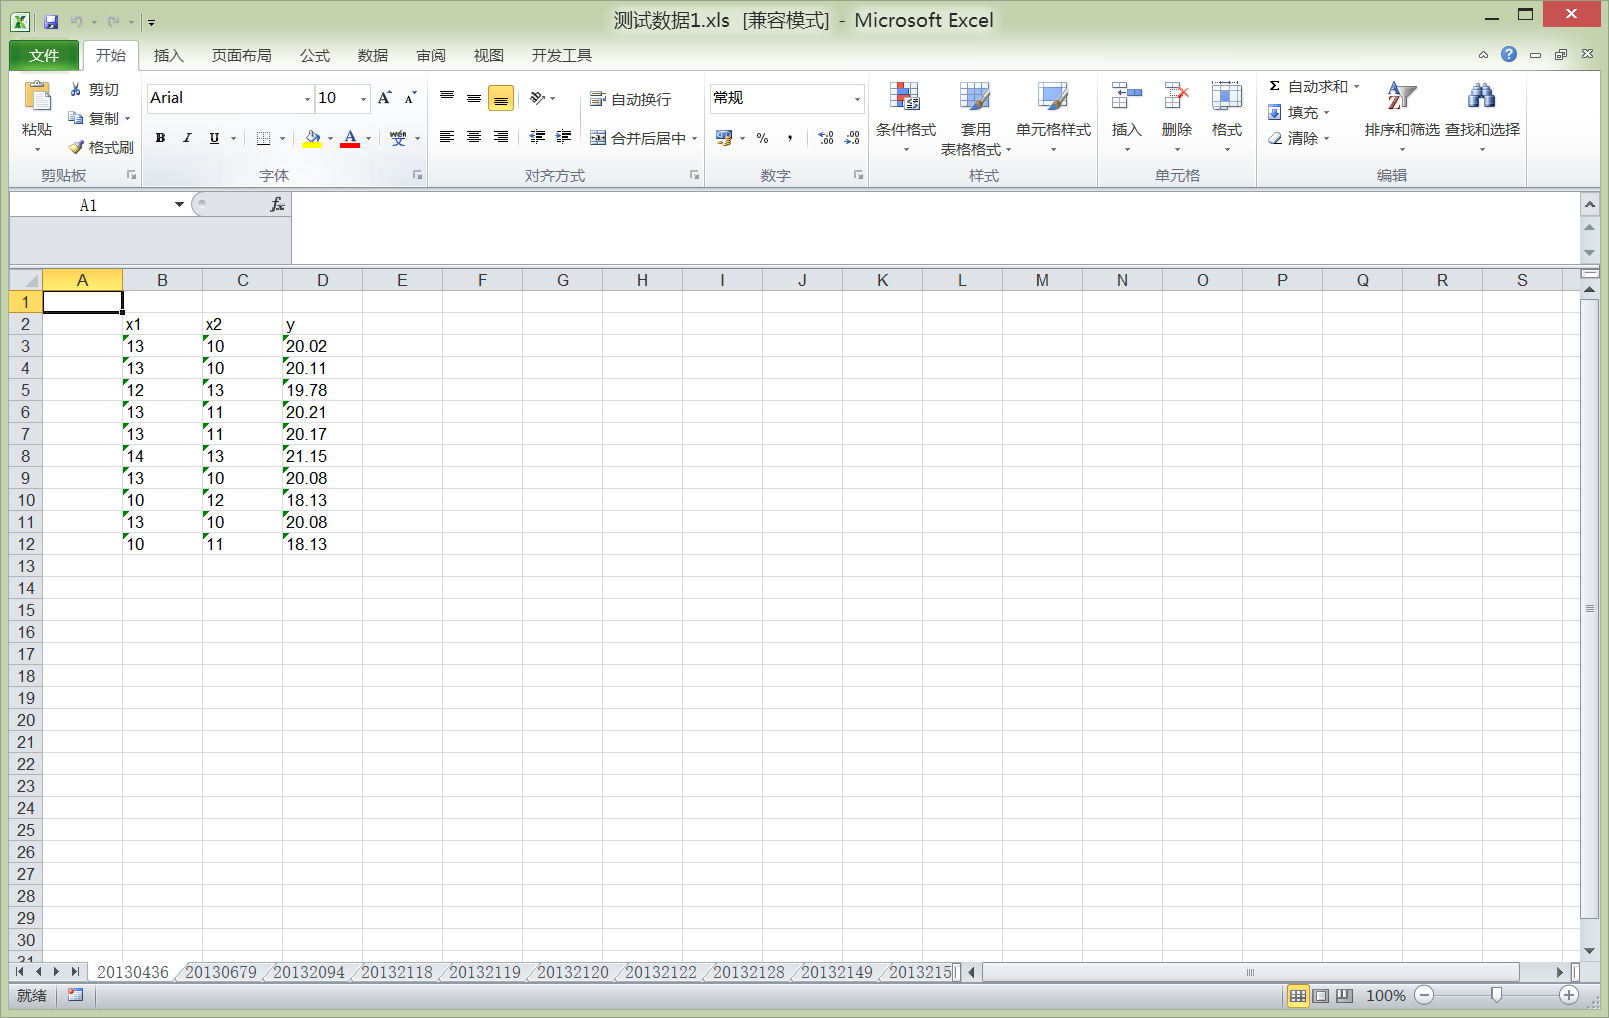
\includegraphics[height=9cm]{images/Link_1.jpg}
            \caption{计量经济学作业一的数据}
            \label{fig:Link_1}
            \end{figure}
            \par
            想到这里,我欣然(屁颠屁颠)的把老师的试题给“解”了,恩对,用程序解的,恩对,批量解的,每个人都有。题型如下图(\ref{fig:Link_2})所示(题目居然要求一步步手工计算,呵呵),我在后面给出了程序,这个程序用来练习MATLAB读取写入excel和MATLAB矩阵操作再合适不过了。
            \begin{figure}[H]
            \centering
            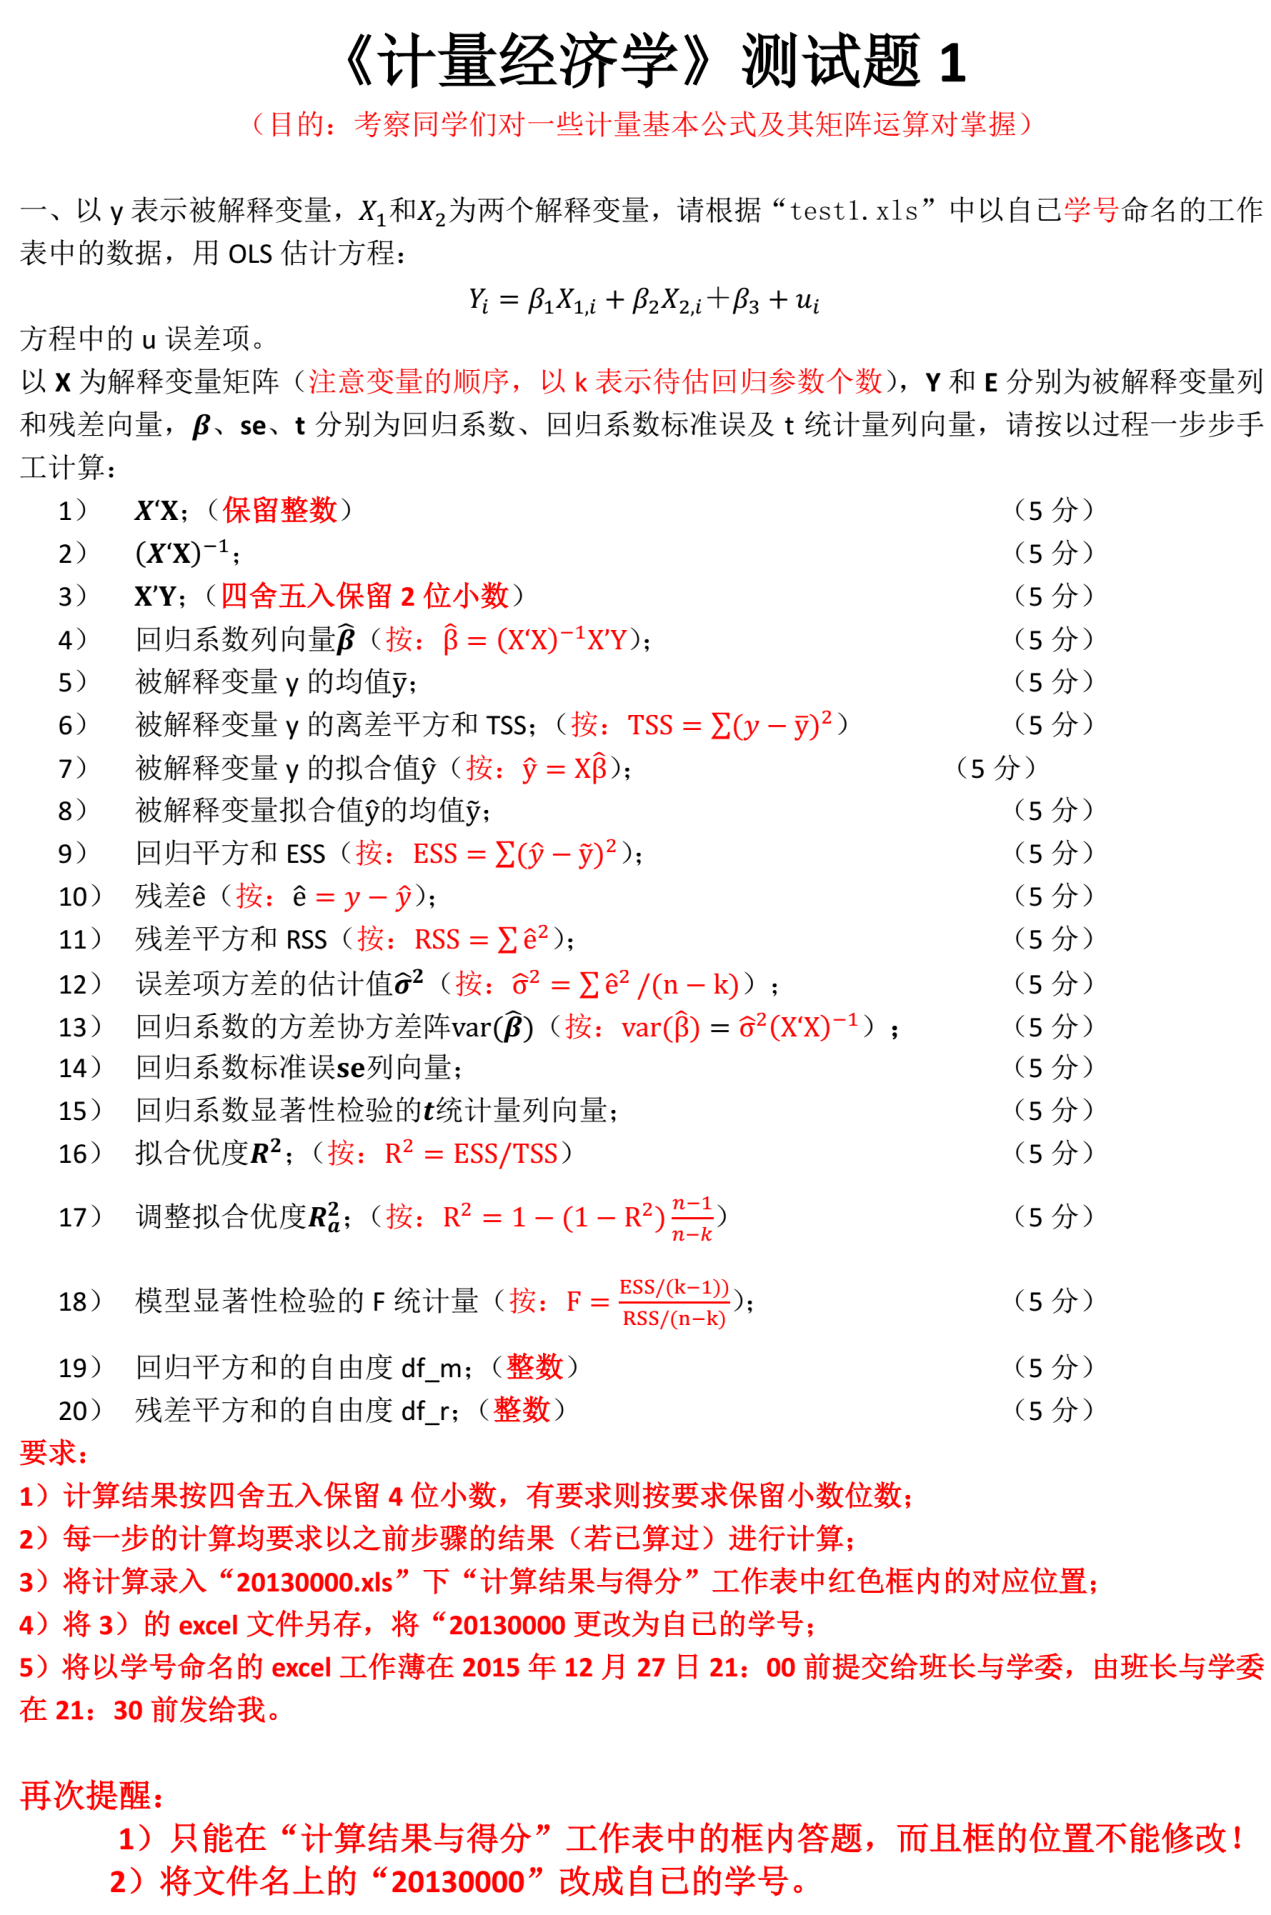
\includegraphics[height=16cm]{images/Link_2.jpg}
            \caption{计量经济学作业一}
            \label{fig:Link_2}
            \end{figure}
            \par
            下面是用于解决《计量经济学》测试题1的程序:$ans\_econom.m$。程序给出了所有试卷的答案,但问题也刚刚开始,可以考虑一下:如何批量生成样本数据,以及如何生成满足不同关系式的样本数据。
            \begin{lstlisting}[language=Matlab]
            %ans_econom.m程序用于解决计量经济学试题1
            clc,clear
            %先用xlsinfo确定有多少个sheet要读
            [Type, Sheet, Format]=xlsfinfo('测试数据1.xls');
            n=length(Sheet);
            for i=1:n
                [~,txt]=xlsread('C:\Users\yanyisong\Documents\MATLAB\测试数据1.xls',Sheet{i},'B3:D12');
               data=[];
                for j=1:size(txt,2)
                    data=[data,str2num(cell2mat(txt(:,j)))];
                end
                X=data(:,1:2);
                X=[X,ones(size(data,1),1)];
                Y=data(:,end);
                T{1}=round(X'*X);%四舍五入取整
                T{2}=roundn(inv(T{1}),-4);
                T{3}=roundn(X'*Y,-2);
                T{4}=roundn(T{2}*T{3},-4);
                T{5}=roundn(mean(Y),-4);
                T{6}=roundn(sum((Y-T{5}).^2),-4);%TSS
                T{7}=roundn(X*T{4},-4);%Yhat
                T{8}=roundn(mean(T{7}),-4);
                T{9}=roundn(sum((T{7}-T{8}).^2),-4);%ESS
                T{10}=roundn(Y-T{7},-4);%error
                T{11}=roundn(sum((T{10}).^2),-4);%RSS
                T{12}=roundn(T{11}/(size(data,1)-size(X,2)),-4);
                T{13}=roundn(T{12}*T{2},-4);
                T{14}=roundn(sqrt(diag(T{13})),-4);
                T{15}=roundn(T{4}./T{14},-4);%H0:beta=0
                T{16}=roundn(T{9}/T{6},-4);
                T{17}=roundn(1-(1-T{16})*(size(data,1)-1)/(size(data,1)-size(X,2)),-4);
                T{18}=roundn(T{9}/(size(X,2)-1)*(size(data,1)-size(X,2))/T{11},-4);
                T{19}=round(size(X,2)-1);
                T{20}=round(size(data,1)-size(X,2));
                height=0;
                for j=1:length(T)
                   xlswrite('20130000.xls',T{j},Sheet{i},['C',num2str(2+height)])
                   height=height+size(T{j},1);
                end
            end
            \end{lstlisting}
            我将上述程序求解的答案放在了20130000.xls中,每个sheet(学号)对应着该学号的答案,结果如下图(\ref{fig:Link_3})所示。
            \begin{figure}[H]
            \centering
            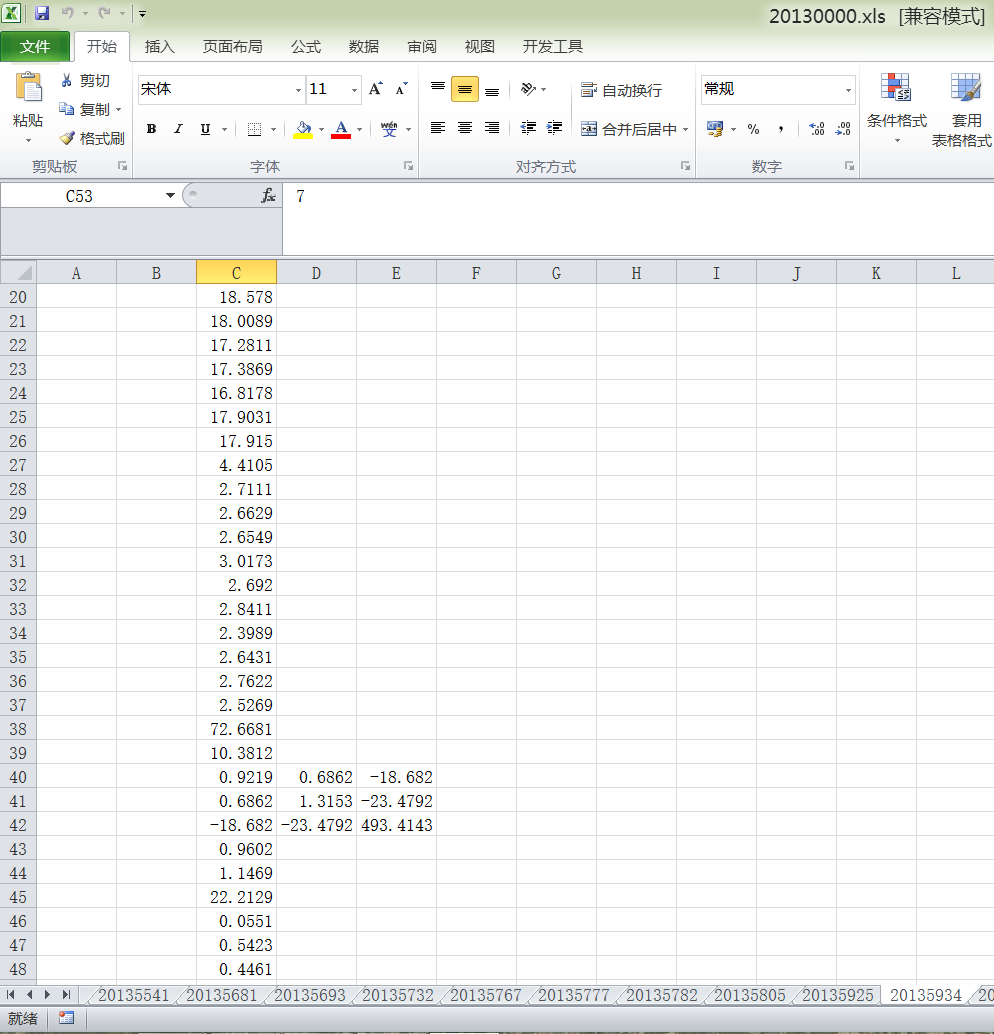
\includegraphics[height=9cm]{images/Link_3.jpg}
            \caption{计量经济学作业1解答}
            \label{fig:Link_3}
            \end{figure}
            \par
            解决测试1之后,我意犹未尽:老师是如何批量生产试卷的呢?每个同学的数据和试题都不一样(这是后面第二份第三份试卷所表现出来的特点),当时,我只解了部分试卷,因为如果要批量解决的话,时间是明显不够的。于是,我决定寒假回家时将问题解决并把试卷也造出来。也就是在造试卷的过程中,我才有幸的结识了COM,COM技术(思想or模式)使得MATLAB能够作为客户来操纵word和excel等COM对象。后来,又在MATLAB link R中再次接触COM和DCOM,RDCOM使得我们能够在MATLAB中调用R(这是令统计人兴奋不已的)。下面,我将简单(真的是很简单)的介绍COM以及ActiveX技术。\\
            \textbf{com介绍}
            \par
            COM(Component Object Model)组件对象模型,COM不是编程语言,他更像是一种规范,一种模式,正如其名“组件对象模型”,他将对象像零件一样的组合在一起,从而形成某些大器件(软件),其所有操作皆是基于对象,流行的组件模型有COM(Component Object Model,对象组件模型)/DCOM(Distributed COM,分布式对象组件模型)和CORBA(Common Object Request Broker Architecture,公共对象请求代理体系结构) 。那么,什么是对象呢?MATLAB(R)中一切皆对象(某矩阵,符号以及某图形等等),对象就是现实中的实体(比如我现在用的这台电脑),我们可以对其进行操作,而容易与对象混淆的是类,类是对象的抽象,是一种抽象的数据类型(MATLAB中用classdef来定义类,《MATLAB面向对象的编程从入门到设计模式》),其实对于类和对象的理解,就像我们汉语所理解的那样,比如“人类”就是一个类,具体的某个人就是“人类”这个类的对象,而“名字、年龄”等就是对象的属性,“宋焱燚、21”就是属性值,人的动作比如“吃饭、穿衣”等就是对象的方法。总之类是对象的模板,对象是类的实例(类就是有相同特征的事物的集合,而对象就是类的一个具体实例)。同时类有多态和继承,例如“人类”可以分为“男人、女人”,“老人、小孩”,那么“男人、女人”就是“人类”的子类。
            \par
            COM对象(组件对象)区别于对象的地方在于“组件”,这些对象能够像零件一样进行组装拼凑,COM对象将其对象的程序进行了封装,我们不需要去读程序然后修改其值,而是直接访问封装后的接口(这个接口也就代表了COM对象),这也是我们访问COM对象(对象的属性、方法和事件)的唯一方法。我们用一个EXCEL来进行举例说明:打开一个EXCEL,下面有工作簿workbook,工作簿下有表sheet,表中有单元格range,一个单元格由4条边框border构成(边框实际上就是线条line),上述的EXCEL、workbook、sheet、range、border均是COM对象,例如,我们可以通过将border对象和其他的底层对象组装,形成单元格range对象;我们可以通过border接口来访问border对象的属性、方法和事件。下面,我们来简单的介绍一下COM对象的属性、方法和时间。
            \par
            \ding{172}COM对象/接口的属性properts:就底层对象边框border而言,我们需要考虑边框的线性、颜色和粗细等,这些就是边框对象的属性,相应的,如果边框对象的属性color是red,那么red就是属性color的属性值。表(\ref{tab:常用的处理对象的属性函数})给出了常用的处理对象的属性函数,其中,如果我们想要查看border对象的线性属性linestyle的可选择的属性值,可以用set函数。
            \begin{table}[H]
            \caption{常用的处理对象的属性函数}
            \label{tab:常用的处理对象的属性函数}
            \centering
            \begin{tabular}{l|l}
                \toprule
                函数 & 描述 \\
                \midrule
            get &一个或多个属性列表和它们的值\\
            set &设置一个或多个属性的值\\
            isprop &确定一个项目是一个COM对象的属性\\
            addproperty &添加一个自定义属性COM对象\\
            deleteproperty &删除一个COM对象的自定义属性\\
            inspect &打开属性检查器来显示和修改属性值\\
            propedit &内置的显示属性页的控制\\
                \bottomrule
            \end{tabular}
            \end{table}
            \par
            \ding{173}COM对象/接口的方法methods:对于workbook对象,我们都可以进行哪些操作?关闭close、打开open、添加add等等,这些操作即为对象的方法method。表(\ref{tab:常用的处理对象的方法函数})给出了常用的处理对象方法函数,如果我们想要调用对象的某种方法,可以使用obj.methodname(arg1,arg2,…)或者是obj.invoke(‘methodname’,arg1,arg2,…)。\\
            注:参数arg应采用枚举法。
            \begin{table}[H]
            \caption{常用的处理对象的方法函数}
            \label{tab:常用的处理对象的方法函数}
            \centering
            \begin{tabular}{l|l}
                \toprule
                函数 & 描述 \\
                \midrule
                methodsview & 图形显示的函数名称和签名\\
                invoke  & 细胞的功能名称和签名,按字母顺序排序\\
                methods & 单元阵列的函数名,按照字母顺序排列的, 大写的名字首先列出来\\
                ismethod & 细胞的功能名称和签名\\
                \bottomrule
            \end{tabular}
            \end{table}
            \par
            \ding{174}COM对象/接口的事件events:在COM中,事件一般是用户启动的某种行为,对于事件,我们应该考虑“某事件发生后,如何处理事件,以及事件带来的后果”。例如:我们单击EXCEL服务器窗口右上角的"X"图标,会关闭EXCEL。单击EXCEL是我们发出的事件,事件发生后触动了事件处理程序(可以想象有一个函数,当时间发生时,就关闭EXCEL),而事件带来的结果就是QUIT EXCEL。表(\ref{tab:常用的处理对象的事件函数})给出了常用的处理对象的事件函数,另外,我们可以编写事件处理程序(event handler functions,可以编写为m函数),并将事件和事件处理程序进行注册/关联(事件event发生时采用该事件处理程序)。
            \begin{table}[H]
            \caption{常用的处理对象的事件函数}
            \label{tab:常用的处理对象的事件函数}
            \centering
            \begin{tabular}{l|l}
                \toprule
                函数 & 描述 \\
                \midrule
                isevent & 判断是否为事件\\
                events & 列出所有的事件\\
                eventlisteners & List event handler functions\\
                registerevent & Associate event handler\\
                unregisterallevents & Unregister all event handlers\\
                unregisterevent & Unregister event handler\\
                \bottomrule
            \end{tabular}
            \end{table}
            \par
            另外,当我们不再需要某COM对象/事件时,可以将其删除(delete)或释放(release),delete用于删除COM对象/事件,而release只能释放COM接口。当删除或关闭一个包含控件的图形窗口figure时,MATLAB会自动释放所有接口。
            \paragraph{COM客户:}我们在使用word时,被视为客户,客户可以要求word服务器来为我们服务些什么(写文档等)。如果我们通过MATLAB来操控word,那么,MATLAB记为word的客户。
            \paragraph{COM服务器:}COM服务器分为进程内和进程外服务器,以dll形式存在的组件对象,在实际调用时,组件代码被载入应用程序中,称为进程内组件(服务器);以exe形式的组件,可以独立运行,称为进程外组件,可以通过actxserver来创建进程内和进程外服务器。MATLAB支持COM技术,也就是说MATLAB可以作为服务器来进行服务,我们可以在excel或word等程序中调用MATLAB。\\
            \textbf{activex介绍}
            \par
            前面我们说到,COM不是一种编程语言而是一种模式,一种规范,它可以重复使用一种COM对象像零件一样用于不同的软件当中,而ActiveX技术是建立在COM之上的。ActiveX 是一个开放的集成平台,使用 ActiveX, 可轻松方便的在 Web页中插入多媒体效果、交互式对象、以及复杂程序。ActiveX组件在MATLAB中可以分为2种情况:ActiveX控件(Active control)和ActiveX 服务器(Active server)。
            \par
            1、ActiveX控件以前称为 OLE 控件或 OCX 控件,用于打包别人编程功能,在 Web页或在其它程序中插入。例如,通过FLASH控件可以使InternetExplorer具有播放动画的能力。在MATLAB中,我们可以向figure窗口中添加ActiveX控件,这是一种可见可嵌入的组件,可以通过actxcontrol、actxcontrollist和actxcontrolselect来创建。
            \par
            2、ActiveX 服务器有两类:进程内服务器(dll动态链接库)和进程外服务器(exe可执行文件),在MATLAB中,我们可以通过actxserver来创建进程内和进程外服务器,例如:用actxserver(‘WMplayer.OCX.8’)来创建一个进程内服务器(组件)Windows Media Player;用actxserver('Excel.Application')来创建一个进程外服务器Excel对象。
            \subsection{com基本命令及例子}
            一个简短的例子
            \begin{lstlisting}[language=Matlab]
            %%%%%%%%%%%%%%%%%%%%%%%%%%%%%%%%%%%%%%%%%%%%%%%%%%%%%%%%%%%%%%%%%%%%%%
            %%%%%%%下面,我们用一个简短的例子来熟悉一下COM的基本操作命令。%%%%%%%%
            %%%%%%%%%%%%%%%%%%%%%%%%%%%%%%%%%%%%%%%%%%%%%%%%%%%%%%%%%%%%%%%%%%%%%%
            Excel = actxserver('Excel.Application')%创建一个Excel对象。
            iscom(Excel)%判断是否为com对象。Excel.iscom。ans=1。
            isinterface(Excel)%判断是否为com接口。Excel.isinterface。ans=0。
            isprop(Excel, 'ActiveSheet')%判断是否为对象/接口的属性
            ismethod(Excel, ' Calculate ') %判断是否为对象/接口的方法
            isevent(Excel, ' NewWorkbook') %判断是否为对象/接口的事件。Excel.isevent
            Excel.inspect %具体显示接口(or COM对象)的属性值和次级接口inspect(e)如下图所示。
            \end{lstlisting}
            \begin{figure}[H]
            \centering
            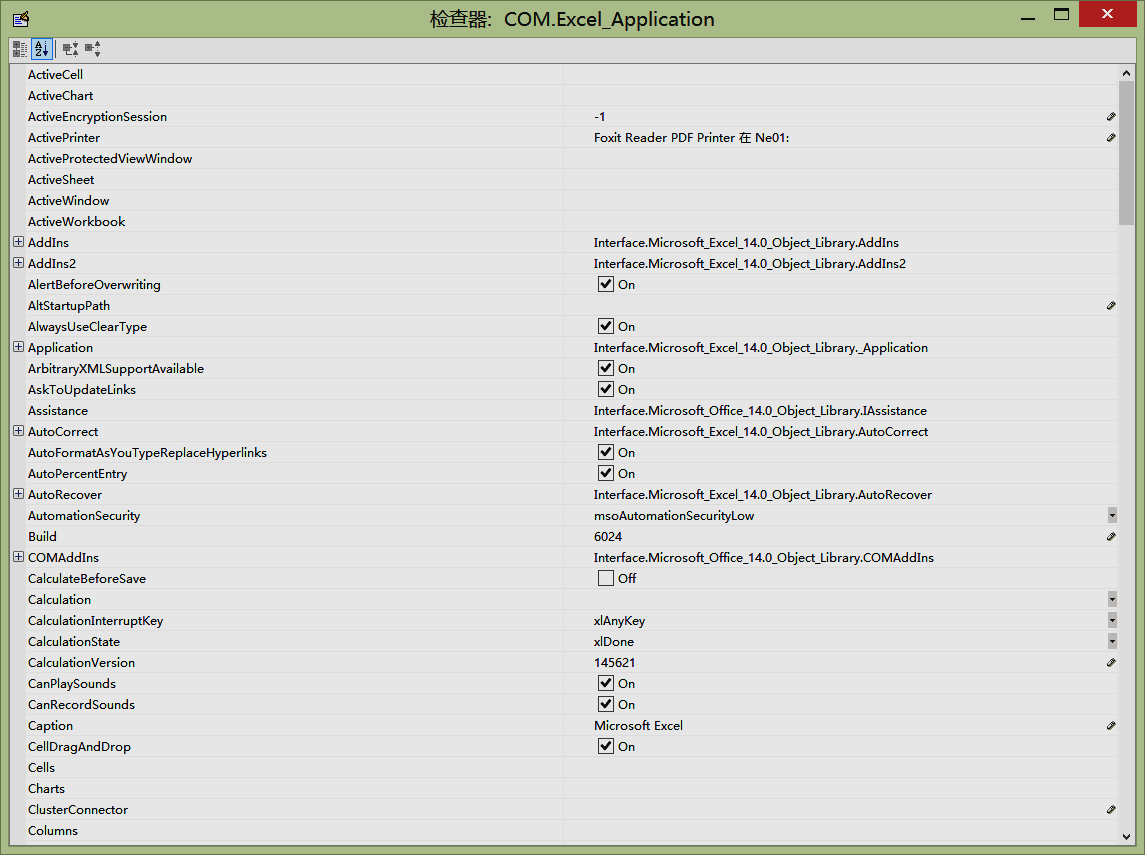
\includegraphics[height=9cm]{images/Link_4.jpg}
            \caption{接口/COM对象的属性值和次级接口inspect}
            \label{fig:Link_4}
            \end{figure}
            Excel.get可以得到接口(or COM对象)的属性值get(e)
            \begin{lstlisting}[language=Matlab]
            >> Excel.get  %得到接口(or COM对象)的属性值get(e)
            Application: [1x1 Interface.Microsoft_Excel_14.0_Object_Library._Application]
            Creator: 'xlCreatorCode'
            Parent: [1x1 Interface.Microsoft_Excel_14.0_Object_Library._Application]
            ActiveCell: []
            \end{lstlisting}
            % \textcolor[rgb]{1.00,0.00,0.00}{图5}
            % \begin{figure}[H]
            % \centering
            % 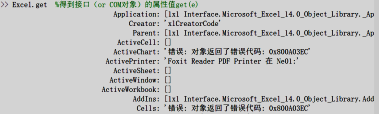
\includegraphics[height=4cm]{images/Link_5.jpg}
            % \label{fig:Link_5}
            % \end{figure}
            Excel.invoke 可得到接口(or COM对象)的方法
            \begin{lstlisting}[language=Matlab]
            >> Excel.invoke
                Calculate = void Calculate(handle)
                DDEExecute = void DDEExecute(handle, int32, string)
                DDEInitiate = int32 DDEInitiate(handle, string, string)
            \end{lstlisting}
            % \textcolor[rgb]{1.00,0.00,0.00}{图6}
            % \begin{figure}[H]
            % \centering
            % 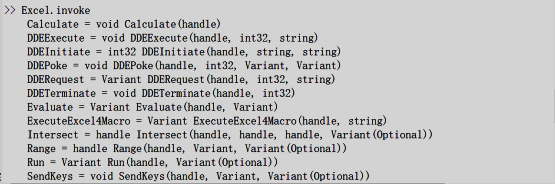
\includegraphics[height=4cm]{images/Link_6.jpg}
            % \label{fig:Link_6}
            % \end{figure}
            Excel.methods 可得到接口(or COM对象)的方法
            \begin{lstlisting}[language=Matlab]
            >> Excel.methods
            ActivateMicrosoftApp            NextLetter
            AddCustomList                   OnKey
            Calculate                       OnRepeat
            CalculateFull                   OnTime
            CalculateFullRebuild            OnUndo
            CalculateUntilAsyncQueriesDone  Quit
            \end{lstlisting}
            % \textcolor[rgb]{1.00,0.00,0.00}{图7}
            % \begin{figure}[H]
            % \centering
            % 
\includegraphics[height=4cm]{images/Link_7.jpg}
            % \label{fig:Link_7}
            % \end{figure}
            Excel.methodsview 可得到接口(or COM对象)的方法methodsview(e),如下图(\ref{接口/COM对象的方法methodsview})所示。
            \begin{figure}[H]
            \centering
            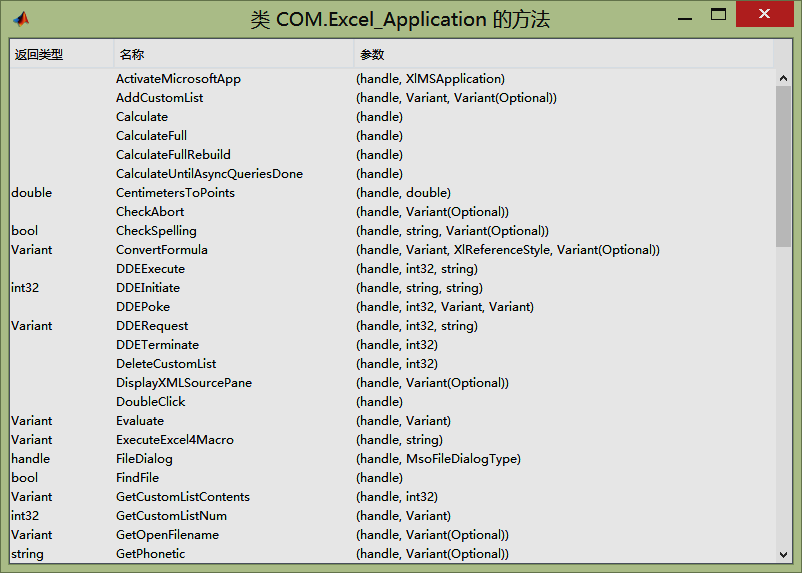
\includegraphics[height=9cm]{images/Link_8.jpg}
            \caption{接口/COM对象的方法methodsview}
            \label{接口/COM对象的方法methodsview}
            \end{figure}
            Excel.events 可得到接口(or COM对象)的事件列表
            \begin{lstlisting}[language=Matlab]
            >> Excel.events %得到接口(or COM对象)的事件列表
                NewWorkbook = void NewWorkbook(handle Wb)
                SheetSelectionChange = void SheetSelectionChange(handle Sh, handle Target)
                SheetBeforeDoubleClick = void SheetBeforeDoubleClick(handle Sh, handle Target, bool Cancel)
                SheetBeforeRightClick = void SheetBeforeRightClick(handle Sh, handle Target, bool Cancel)
            \end{lstlisting}
            % \textcolor[rgb]{1.00,0.00,0.00}{图9}
            % \begin{figure}[H]
            % \centering
            % 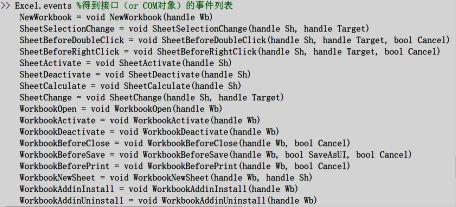
\includegraphics[height=4cm]{images/Link_9.jpg}
            % \label{fig:Link_9}
            % \end{figure}
            % \textcolor[rgb]{1.00,0.00,0.00}{Excel. eventlisteners $\%$事件的列表 eventlisteners(Excel)}\\
            % \textcolor[rgb]{1.00,0.00,0.00}{图10}
            \begin{lstlisting}[language=Matlab]
            %查看属性Cursor的所有可选属性值。Excel.set('属性', '属性值')
            set(Excel, 'Cursor')
            ans =
                'xlIBeam'
                'xlDefault'
                'xlNorthwestArrow'
                'xlWait'
            Excel.Cursor = 'xlDefault'; %重置光标。
            Excel.Visible = 1;    % 设置Excel属性为可见。set(Excel, 'Visible', 1);
            %wdata = Open(Excel,'c:\work\weekly_log.xlsx'); % 连接到现有Excel应用程序
            eWorkbook = Excel.Workbooks.Add; %添加一个工作簿。Add(Excel.Workbooks);
            eSheets = Excel.ActiveWorkbook.Sheets;%活动的工作簿的表
            eSheet1 = eSheets.get('Item',1);%活动的工作簿的第一张表eSheet1 = Item(eSheets,1);
            eSheet1.Activate%使第一张工作表活跃
            eNewSheet = Add(eSheets,[],eSheet1); %通过使用一个空数组[]。
            \end{lstlisting}
            \begin{figure}[H]
            \centering
            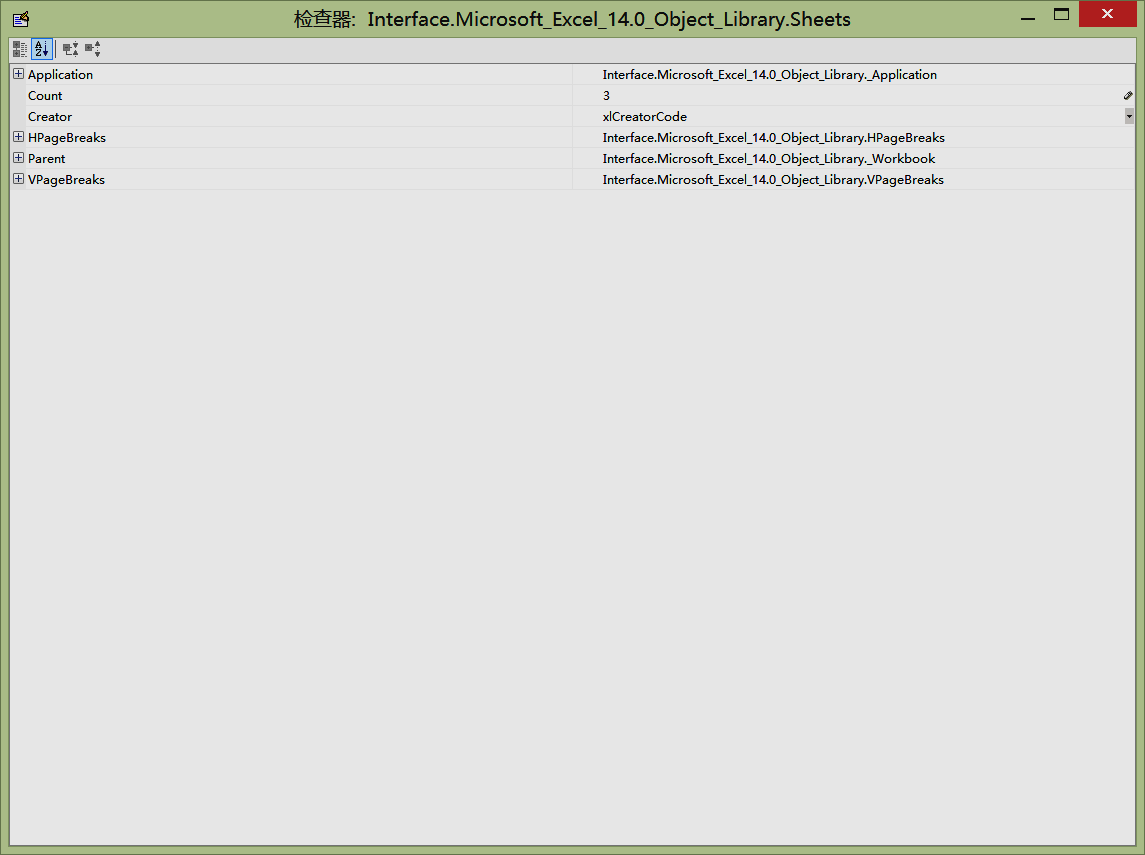
\includegraphics[height=9cm]{images/Link_11.jpg}
            \label{fig:Link_11}
            \end{figure}
            \begin{lstlisting}[language=Matlab]
            ws = Excel.Activesheet;%正在活动的表
            ws.StandardHeight  %显示工作表中的所有行的默认高度。ans = 14.4000
            methods(ws, '-full') %显示语法创建一个函数{}范围{}对象。}
            wsRange = ws.Range('A1');%得到A1单元格
            wsRange.RowHeight = 25; %增加行高。
            %将MATLAB数据保存到工作表。
            A = [1 2; 3 4];
            eActivesheetRange = get(ws,'Range','A1:B2');
            eActivesheetRange.Value = A;
            %读取excel数据到MATLAB
            eRange = get(e.Activesheet,'Range','A1:B2');
            B = eRange.Value;
            B = reshape([B{:}],size(B)); %将数据转换成一个双矩阵。
            %% 为工作簿OnClose事件显示消息
            %{
            在当前文件夹, 创建以下事件处理程序文件:OnBeforeCloseWorkbook.m ,。
            function OnBeforeCloseWorkbook(varargin)
            disp('BeforeClose event occurred')
            %}
            registerevent(hWorkbook,{'BeforeClose' @OnBeforeCloseWorkbook})%注册函数为 OnClose 事件。
            SaveAs(eWorkbook,'myfile.xls') %保存工作簿文件中。
            eWorkbook.Saved = 1; %保存文件
            Close(eWorkbook) %关闭工作簿。
            BeforeClose event occurred
            Quit(Excel) %退出Excel程序
            eWorkbook.release  %释放接口
            Excel.delete   %删除接口delete(Excel)
            %%%%%%%%%%%%%%%%%%%%%%%%%%%%%%%%%%%%%%%%%%%%%%%%%%%%%%%%%%%%%%%%%%%
            \end{lstlisting}
            % \textcolor[rgb]{1.00,0.00,0.00}{图12}
            % \begin{figure}[H]
            % \centering
            % 
\includegraphics[height=1cm]{images/Link_12.jpg}
            % \label{fig:Link_12}
            % \end{figure}
    \subsection{操作案例}
        \par
        下面,我们将利用COM技术来实现一个稍微复杂一点的例子。在这个例子中,我们将用MATLAB来批量生产试卷(没错啦,就是我寒假回家做的),试卷的样式仿照《计量经济学测试2》(具体内容在相关文件夹下):有一个总的压缩文件“计量经济学2.rar”,里面每一个学号对应一个压缩文件(20135064.rar),每个学号的压缩文件夹下有相应的数据、试卷以及答题卡(企业数据.dta 、20130436.pdf和20130436.xlsx),试卷的内容如图(\ref{fig:试卷的内容})所示。
        % \textcolor[rgb]{1.00,0.00,0.00}{试卷的内容}
        \begin{figure}[H]
        \centering
        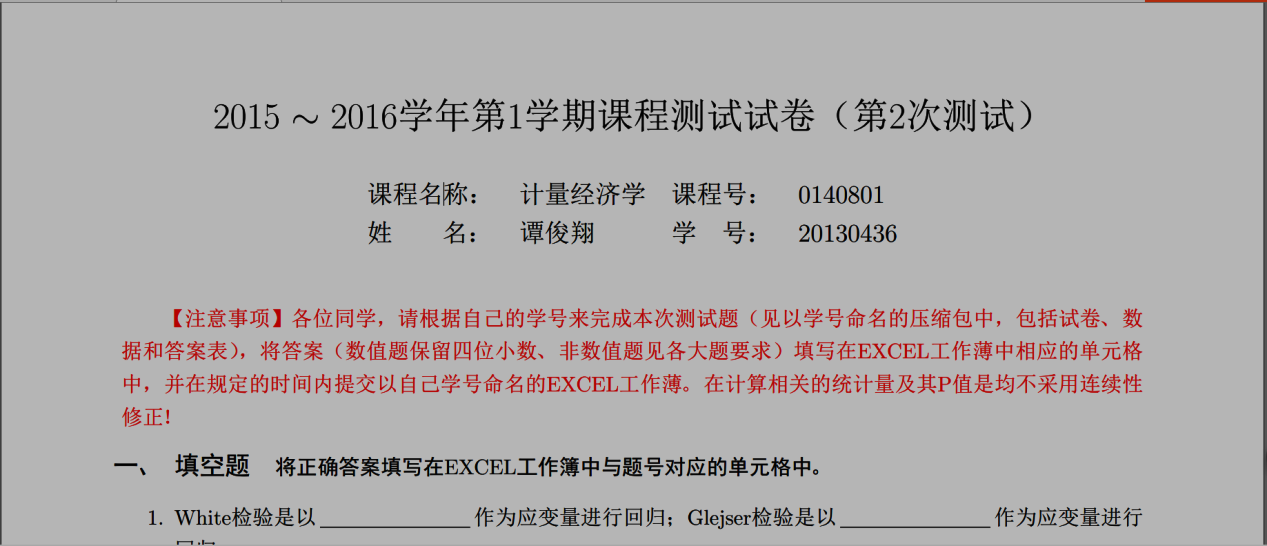
\includegraphics[height=6cm]{images/Exam_content.jpg}
        \caption{试卷的内容}
        \label{fig:试卷的内容}
        \end{figure}
        \par
        首先,我们来想象一下,如果是人工设计试卷的话都有哪些过程。由于每份试卷的题目都不相同,可以猜到,试卷应该是从题库中抽取出来的(题库应该具有可变性)。我们就某位同学的试卷而言:1、需要把试卷的通用格式(例如:标题、前言、版面和注意事项等等)设定好。2、对于试卷的试题内容,我们随机的从题库中抽取部分题目,复制粘贴到WORD试卷上,同时,我们还应该记录抽取题目的答案,以用于日后的批改工作。
        \par
        然后,我们来捋一捋在设计程序时,应该做哪些内容。
        \begin{enumerate}
          \item 设计试卷(doc格式)的通用格式。由于从整体上看,每个同学的试卷的通用格式是相似的,只是试题的内容不同,所以我们先来设定试卷的通用格式。
          \item 设计答案和答题卡(xls格式)的通用格式。由于我们并不知道每张试卷的题目数量,所以我们并不能标注具体的题号以及题号对应的答案,只有从题库抽取题目的时候,我们才能标记答案,因此,我们先设定答案和答题卡的通用格式(例如:某单元格的格式)。
          \item 读取题库(题库是自制的)。在读取题库时,我们要记录题库中有哪些题型,以及各题型的数量。同时,题库中应有每题的答案。
          \item 设计试卷试题内容以及保存答案(抽选题目)。从题库的各个题型中选取部分试题作为试卷的内容,并记录抽到的试题的答案,将答案抹去,作为答题卡。
          \item 保存试卷、答案以及答题卡。将doc格式的试卷保存,并另存为pdf格式的试卷,保存xls格式的答题卡。将doc、pdf和xls答题卡保存在对应的学号下的文件夹里(不存在文件夹时要创建),并压缩文件夹。将xls格式的答案单独保存到某文件夹,以备后用。
        \end{enumerate}
        \par
        最后,我们写一写上面过程的注意事项以及后续工作(待完成)。
        \begin{enumerate}
          \item 答案和答题卡的xls有两种方式。一种方式是一个学号一个xls,另一种方式是只有一个xls而每个学号对应一个sheet。
          \item 复制答案和答题卡。如果所有人的数据以及试题是一样的,那么在设置第一位同学的答案和答题卡之后,后面同学的可以复制而来。
          \item 有不同题型的答案,如何保存答案可以使后面的批题工作更简单?
          \item 模拟批题的过程,假设有一份答案,我们如何进行批题工作?写出相应的程序。
          \item 能否设置多选题的批题方式,使得可以存在两种情况:一种情况是错选不得分,另一种情况是多选不得分?(如果你对试卷还有其他的要求,请自行补充)。
        \end{enumerate}
        \par
        下面,给出试卷的程序examinationpape.m。examinationpape.m是用于生产某学号的试卷、答案以及答题卡,并保存。如果想要批量生产,可以运行manypaper.m函数。
        \subsubsection{1、函数examinationpape.m的输入}
            \begin{lstlisting}[language=Matlab]
            function examinationpaper(Visible, Margin, title, classname, classnumber, name, studentnumber, annomcement,...
                selectnumber, cancopy, cardtype, pwd)
            % 此函数用于从已有题库中抽取部分题目生成word or pdf文档
            % 输入参数nargin说明:
            % visible : 文档是否显示出来 1显示(bool)。默认:0
            % margin : 页面边距 (margin为4值向量array)。默认:[60, 45, 45, 45];
            % title : 文档标题(string)。默认:['2015~2016学年第一学期课程测试试卷(第2次测试)'];
            % classname : 课程名称(string)。默认: '计量经济学';
            % classnumber :课程号(string)。默认:'0140801';
            % name : 学生姓名(string)。默认:'宋焱燚';
            % studentnumber : 学号(string)。默认:'20135064';
            % annomcement : 注意事项(string)。默认:
            % selectnumber : 各题选择个题数(4 array)。默认:[3, 5, 5, 5]
            % cancopy : 答题卡能否复制(bool)1能。默认:0
            % cardtype:答题卡的类型(int)。默认:0为一个学号一张答题卡(.xls),1表示所有答题卡在一个.xls中
            % pwd:试卷路径(string)。默认: 'D:\Program Files\MATLAB\R2014a\work\20计量经济作业解\生成的试卷';
            \end{lstlisting}
        \subsubsection{2、设置默认参数}
            \begin{lstlisting}[language=Matlab]
            %%%%%%%%%%%%%%%%%设置默认参数%%%%%%%%%%%%%%%%%
            if nargin < 1
                Visible = 0;
            end
            if nargin < 2
                Margin = [60, 45, 45, 45];
            end
            if nargin < 3
                title = ['2015~2016学年第一学期课程测试试卷(第2次测试)'];
            end
            if nargin < 4
                classname = '计量经济学';
            end
            if nargin < 5
                classnumber = '0140801';
            end
            if nargin < 6
                name = '宋焱燚';
            end
            if nargin < 7
                studentnumber = '20135064';
            end
            if nargin < 8
                annomcement =  ['【注意事项】各位同学,请根据自己的学号来完成本次测试题(见以学号命名的压缩包中,包括试卷、数据和答案表),将答案(数值题保留四位小数、非数值题见各大题要求)填写在EXCEL工作薄中相应的单元格中,并在规定的时间内提交以自己学号命名的EXCEL工作薄。在计算相关的统计量及其P值时均不采用连续性修正!'];
            end
            if nargin < 9
                selectnumber = [3, 5, 5, 5] ;%选题数量
            end
            if nargin < 10
                cancopy = 0;
            end
            if nargin <11
                cardtype = 0;
            end
            if nargin < 12
                pwd = 'D:\Program Files\MATLAB\R2014a\work\20计量经济作业解\生成的试卷';
            end
            \end{lstlisting}
        \subsubsection{3、设置试卷通用格式.doc}
            此部分是用于设计试卷的通用格式,设计的格式如图(\ref{fig:试卷的通用格式})所示。
            \begin{lstlisting}[language=Matlab]
            %%%%%%%%%%%%%%%%%设置试卷通用格式.doc%%%%%%%%%%%%%%%%
            % 设定测试Word文件名和路径
            %pwd = 'D:\Program Files\MATLAB\R2014a\work\20计量经济作业解\生成的试卷';
            filespec_user = [pwd '\' studentnumber '\' studentnumber '.doc'];
            % 判断Word是否已经打开,若已打开,就在打开的Word中进行操作,否则就打开Word
            try
                Word = actxGetRunningServer('Word.Application');% 若Word服务器已经打开,返回其句柄Word
            catch
                Word = actxserver('Word.Application'); % 创建一个Microsoft Word服务器,返回句柄Word
            end
                                                     %Visible = 1;
            Word.Visible = Visible;    % 设置Word属性为可见。
            % 若测试文件存在,打开该测试文件,否则,新建一个文件,文件名为测试.doc
            if exist(filespec_user, 'file') == 2
                %file:文件
                Document = Word.Documents.Open(filespec_user);% Document = invoke(Word.Documents,'Open',filespec_user);
            else
                Document = Word.Documents.Add; % Document = invoke(Word.Documents, 'Add');
            end
            Paragraph = Document.Paragraphs; %返回段落接口句柄
            Content = Document.Content;    % 返回Content接口句柄
            Selection = Word.Selection;    % 返回Selection接口句柄
            Paragraphformat = Selection.ParagraphFormat;  % 返回ParagraphFormat接口句柄
            % 页面设置
            %Margin = [60, 45, 45, 45];
            Document.PageSetup.TopMargin =  Margin(1) ;      %上边距60磅
            Document.PageSetup.BottomMargin = Margin(2) ;   %下边距45磅
            Document.PageSetup.LeftMargin =  Margin(3) ;     %左边距45磅
            Document.PageSetup.RightMargin = Margin(4) ;    %右边距45磅
            %
            % 设定文档内容的起始位置和标题
            Content.Start = 0;         % 设置文档内容的起始位置
            %title = ['2015~2016学年第一学期课程测试试卷(第2次测试)'];
            Content.Text = title;      % 输入文字内容
            Content.Font.Size = 16 ;   % 设置字号为16(3号字体)
            Content.Font.Bold = 4 ;    % 字体加粗
            Content.Paragraphs.Alignment = 'wdAlignParagraphCenter';    % 居中对齐
            Content.Paragraphs.SpaceBefore = 12;   %文档内容.段落.段前间距 =12磅
            Content.Paragraphs.SpaceAfter = 12;   %文档内容.段落.段后间距 =12磅
            %
            Selection.Start = Content.end;    % 设定下面内容的起始位置
            Selection.TypeParagraph;    % 回车,另起一段
            %Selection.TypeParagraph;
            Content.Start = Selection.end;
            classname1 = ['  ', classname, '  '];
            classnumber1 =['  ', classnumber, '  '];
            name1 = ['  ', name, ' '];
            studentnumber1 = ['  ', studentnumber, '  ' ];
            information1 = ['  课程名称:',classname1,'  课程号: ',classnumber1];
            Content.Text = information1;
            Content.Font.Size = 12;   % 设置字号为12(小四号字体)
            Content.Font.Bold = 0;    % 字体不加粗
            Content.Paragraphs.Alignment = 'wdAlignParagraphCenter';    % 居中对齐
            Content.Paragraphs.SpaceBefore = 0;   %文档内容.段落.段前间距 =0磅
            Content.Paragraphs.SpaceAfter = 0;   %文档内容.段落.段后间距 =0磅
            %
            Selection.Start = Content.end;
            Selection.TypeParagraph;
            Content.Start = Selection.end;
            information2=['  学生姓名: ',name1,'  学号: ', studentnumber1];
            Content.Text = information2;
            Content.Paragraphs.SpaceBefore = 0;   %文档内容.段落.段前间距 =0磅
            Content.Paragraphs.SpaceAfter = 0;   %文档内容.段落.段后间距 =0磅
            %
            Selection.Start = Content.end;
            Selection.TypeParagraph;
            %Selection.TypeParagraph;
            Content.Start = Selection.end;
            %annomcement = ['【注意事项】各位同学,请根据自己的学号来完成本次测试题(见以学号命名的压缩包中,包括试卷、数据和答案表),将答案(数值题保留四位小数、非数值题见各大题要求)填写在EXCEL工作薄中相应的单元格中,并在规定的时间内提交以自己学号命名的EXCEL工作薄。在计算相关的统计量及其P值时均不采用连续性修正!'];
            Content.Text = annomcement;
            Content.Font.ColorIndex = 'wdRed';
            Content.Font.Size = 10.5; % 设置字号为10.5(5号字体)
            Content.Paragraphs.Alignment =  'wdAlignParagraphLeft';
            Content.Paragraphs.FirstLineIndent = 0;
            Content.Paragraphs.SpaceBefore = 12;   %文档内容.段落.段前间距 =12磅
            Content.Paragraphs.SpaceAfter = 12;   %文档内容.段落.段后间距 =12磅
            Selection.Start = Content.end;
            Selection.TypeParagraph;
            \end{lstlisting}
            \begin{figure}[H]
            \centering
            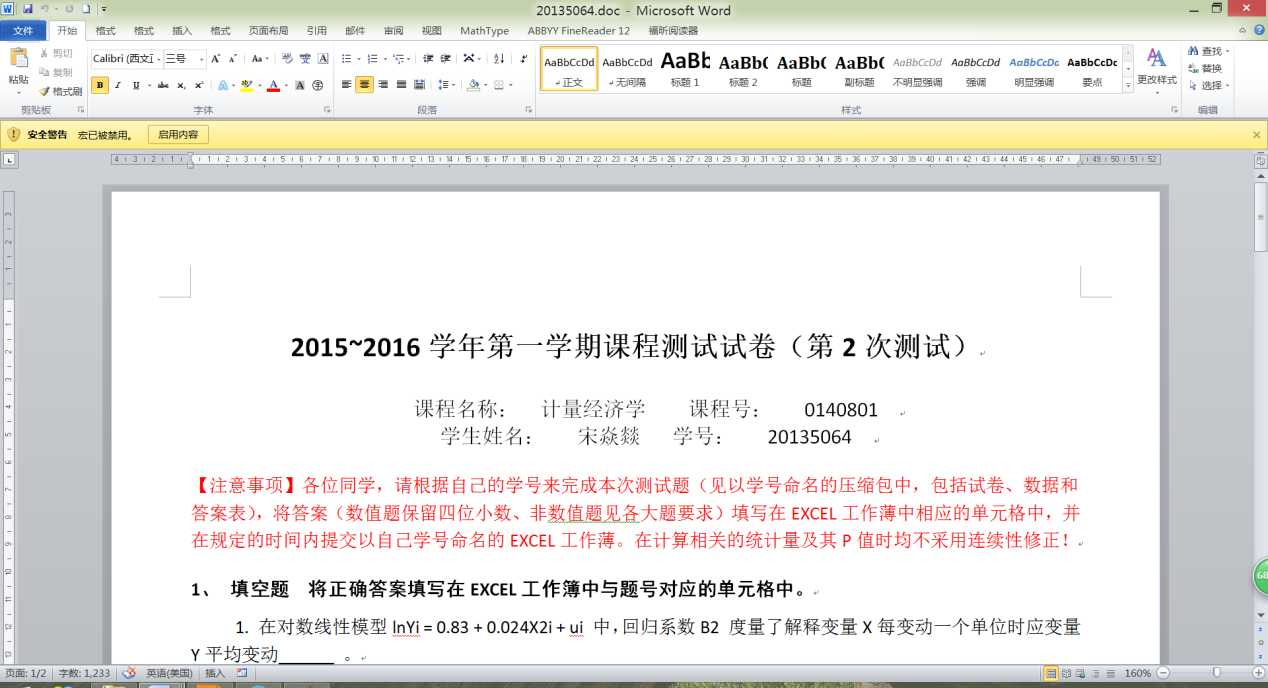
\includegraphics[height=8cm]{images/examination_paper_common_format.jpg}
            \caption{试卷的通用格式}
            \label{fig:试卷的通用格式}
            \end{figure}
        \subsubsection{4、答案和答题卡}
            此部分是用于生成答案和答题卡的通用格式。
            \begin{lstlisting}[language=Matlab]
            %%%%%%%%%%%%%%%%%创建EXCEL :答案和答题卡%%%%%%%%%%%%%%%%%%%%
            %%%%%%%%%%%%1、答题卡xls%%%%%%%%%%%
            if cardtype == 1
                filespec_user2 = [pwd, '\答题卡和答案\答题卡.xls'];% 设定测试Excel文件名和路径
                %如果答题卡(EXCEL)是类型1(所有答题卡只在一个*.xls中,只是sheet的名称为学号)
                %打开EXCEL
                Excel = actxserver('Excel.Application');
            %{
            %不能够用下面方法,因为我们打开了两个EXCEL对象
                try
                    Excel = actxGetRunningServer('Excel.Application');
                catch
                    Excel = actxserver('Excel.Application');
                end
            %}
            else
                filespec_user2 = [pwd, '\', studentnumber, '\', studentnumber '.xls'];
                Excel = actxserver('Excel.Application');
            end
            Excel.Visible = Visible;
            % 创建工作簿workbook
            if exist(filespec_user2, 'file') == 2
                Workbook = Excel.Workbooks.Open(filespec_user2);
            else
                Workbook = Excel.Workbooks.Add;
            end
            %创建工作表
            if  strcmp(Workbook.Sheets.Item(1).Name, 'Sheet1')
                Sheet = Workbook.Sheets.Item(1);
                Workbook.Sheets.Item(2).Delete;
                Workbook.Sheets.Item(2).Delete;
                %Sheet.Active;
                Sheet.Name = studentnumber;
            elseif  cancopy ==1
                 sheetnum = Workbook.Sheets.Count;
                 Sheet = Workbook.ActiveSheet.Copy([], Workbook.Sheets.Item(sheetnum));
                 Sheet.Name = studentnumber;
            else
                 sheetnum = Workbook.Sheets.Count;
                 Sheet = Workbook.Sheets.Add([], Workbook.Sheets.Item(sheetnum), 1, []);
                 Sheet.Name = studentnumber;
            end
            %单元格设置
            if cancopy == 0
                Sheet.Range('B2:C2').Border.Weight = 2;
                Sheet.Range('B2:C2').Border.ColorIndex = 23;
                Sheet.Range('B2:C2').Border.LineStyle = 9;
                Sheet.Range('B2:C2').Font.Size = 12;
                Sheet.Range('B2:C2').Font.bold = 2;
                Sheet.Range('B2:C2').Font.Name = '黑体';
                Sheet.Range('B2:C2').HorizontalAlignment = 3;
                Sheet.Range('B2:C2').VerticalAlignment = 2;
                Sheet.Range('B2').Value = '题号';
                Sheet.Range('C2').Value = '答案';
            end
            %%%%%%%%%%%%2、答案xls%%%%%%%%%%%%%%
            if cardtype == 1
                %如果答题卡(EXCEL)是类型1(所有答题卡只在一个*.xls中,只是sheet的名称为学号)
                filespec_user3 = [pwd, '\答题卡和答案\答案.xls'];
                Excel2 = actxserver('Excel.Application');%打开EXCEL
            %{
                try
                    Excel2 = actxGetRunningServer('Excel.Application');
                catch
                    Excel2 = actxserver('Excel.Application');
                end
            %}
            else
                filespec_user3 = [pwd, '\答案\', studentnumber, '.xls'];
                Excel2 = actxserver('Excel.Application');
            end
            Excel2.Visible = Visible;    % 设置Excel服务器为可见状态
            % 创建工作簿workbook
            if exist(filespec_user3, 'file') == 2
                Workbook2 = Excel2.Workbooks.Open(filespec_user3);
            else
                Workbook2 = Excel2.Workbooks.Add;
            end
            %创建工作表
            if  strcmp(Workbook2.Sheets.Item(1).Name, 'Sheet1')
                Sheet2 = Workbook2.Sheets.Item(1);
                Workbook2.Sheets.Item(2).Delete;
                Workbook2.Sheets.Item(2).Delete;
                %Sheet2.Active;
                Sheet2.Name = studentnumber;
            elseif  cancopy ==1
                 sheetnum2 = Workbook2.Sheets.Count;
                 Sheet2 = Workbook2.ActiveSheet.Copy([], Workbook2.Sheets.Item(sheetnum2));
                 Sheet2.Name = studentnumber;
            else
                 sheetnum2 = Workbook2.Sheets.Count;
                 Sheet2 = Workbook2.Sheets.Add([], Workbook2.Sheets.Item(sheetnum2), 1, []);
                 Sheet2.Name = studentnumber;
            end
            %单元格设置
            if cancopy == 0
                Sheet2.Range('B2:C2').Border.Weight = 2;
                Sheet2.Range('B2:C2').Border.ColorIndex = 23;
                Sheet2.Range('B2:C2').Border.LineStyle = 9;
                Sheet2.Range('B2:C2').Font.Size = 12;
                Sheet2.Range('B2:C2').Font.bold = 2;
                Sheet2.Range('B2:C2').Font.Name = '黑体';
                Sheet2.Range('B2:C2').HorizontalAlignment = 3;
                Sheet2.Range('B2:C2').VerticalAlignment = 2;
                Sheet2.Range('B2').Value = '题号';
                Sheet2.Range('C2').Value = '答案';
            end
            \end{lstlisting}
        \subsubsection{5、读取题库}
            题库是我们仿照《计量经济学测试2》里面的试题给出的,题库的样式如图(\ref{fig:题库})所示,题库中应该存在题型、题号、题目和答案4个部分,允许添加和删除题目,允许添加和删除题型。
            % \textcolor[rgb]{1 0 0}{图:题库}
            \begin{figure}[H]
            \centering
            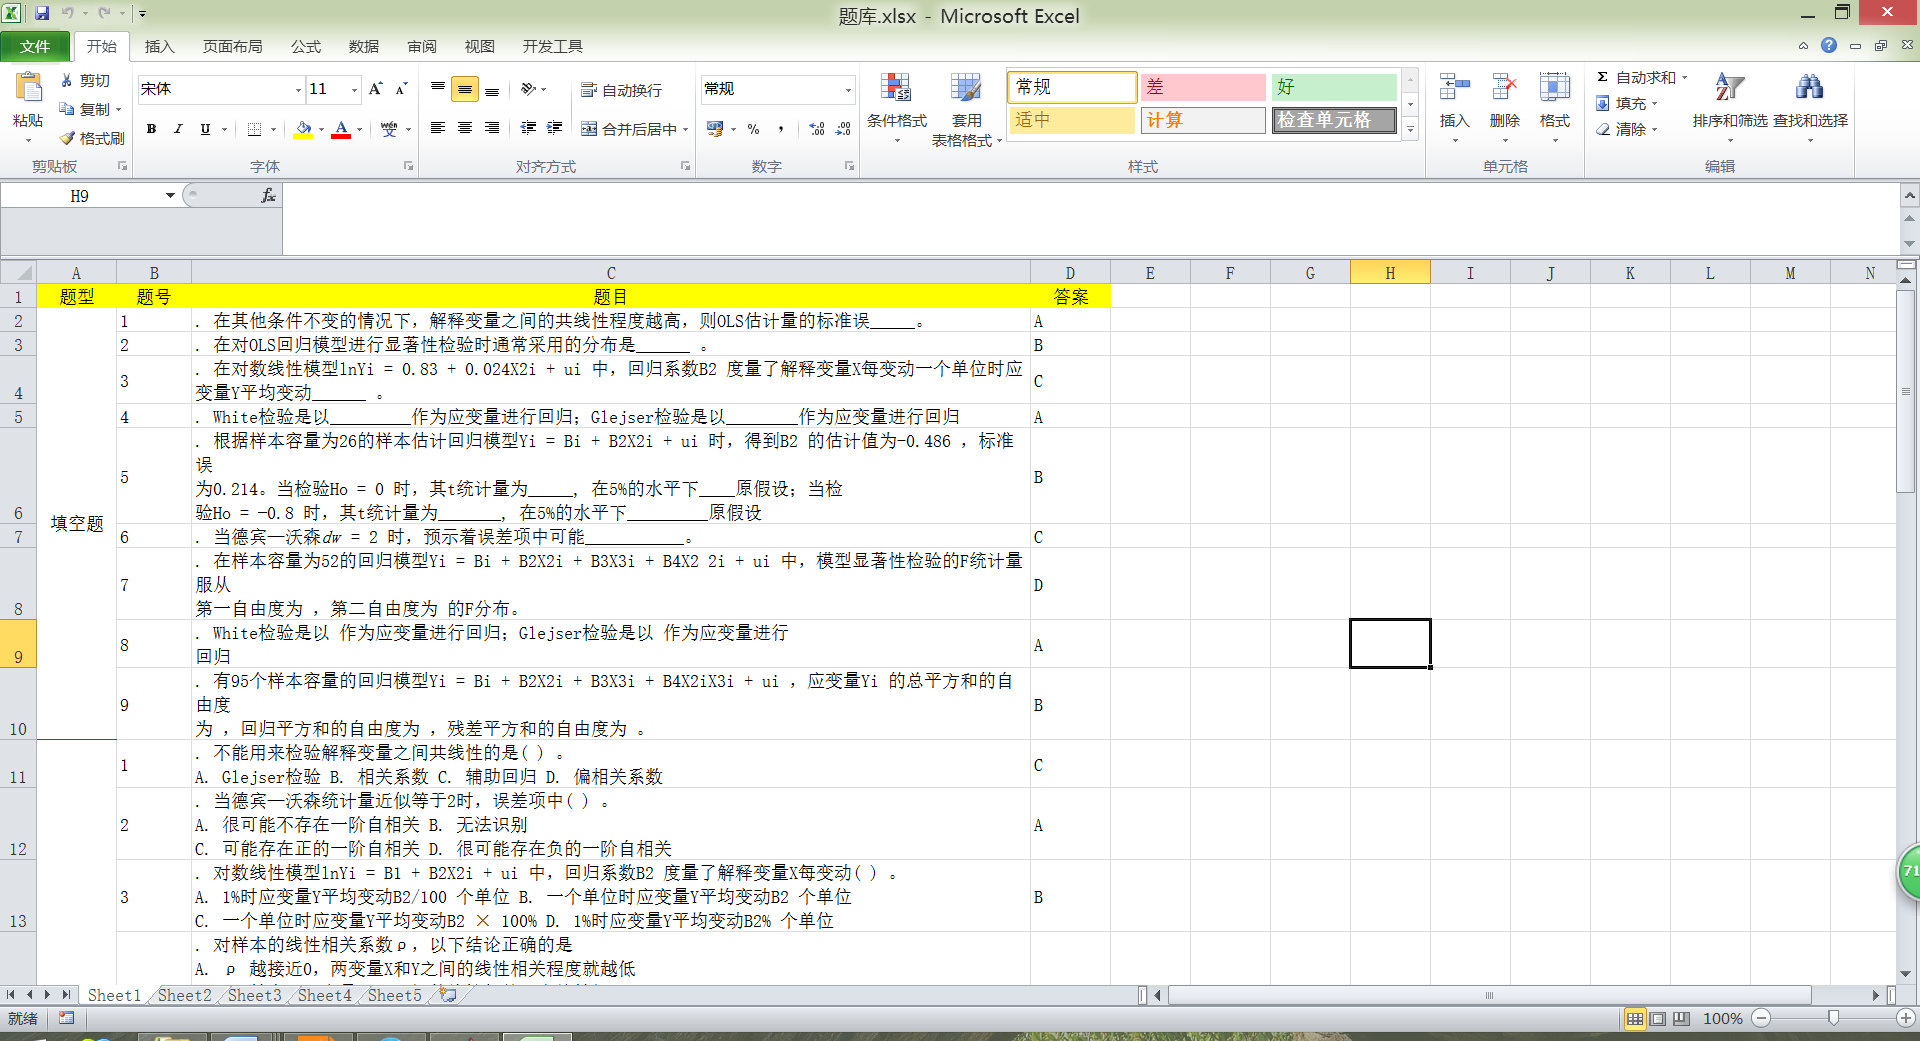
\includegraphics[height=8cm]{images/QB.jpg}
            \caption{题库}
            \label{fig:题库}
            \end{figure}
            \begin{lstlisting}[language=Matlab]
            %%%%%%%%%%%%%%%读取题库(可以写到函数外面)%%%%%%%%%%%%%%%%%%%%%%
            if ~exist('alldata') %如果不存在变量alldata
                [num, txt, alldata] =  xlsread('D:\Program Files\MATLAB\R2014a\work\20计量经济作业解\题库.xlsx', 1);%应该将题库一直打开
                txt(1, :) = [];
                count = find(num == 1);
                typeoftopic = txt(count, 1);%题型
            end

            for i=1:length(count)
                if i ~= length(count)
                    numoftopic(i) = count(i+1) - count(i);%各题型数量
                else
                     numoftopic(i) = length(num) - count(i) + 1;
                end
            end
            \end{lstlisting}
        \subsubsection{6、设计试卷试题内容并记录答案}
            此部分用于从题库中抽取部分试题作为试卷的内容,并记录题目对应的题号和答案。
            \begin{lstlisting}[language=Matlab]
            %%%%%%%%%%%%%%%设计试卷试题内容并记录答案%%%%%%%%%%%%%%%%%%%%%%
            %selectnumber = [3 5 5 5] ;%选题数量
            ind = 0;
            for i = 1:length(count)
                Title=[num2str(i),'、 ',typeoftopic{i},'  将正确答案填写在EXCEL工作簿中与题号对应的单元格中。'];
                Content.Start = Selection.end;
                Content.Text = Title;
                Content.Font.ColorIndex = 'wdBlack';
                Content.Font.Size = 11 ;   % 设置字号为11(3号字体)
                Content.Font.Bold = 4;    % 字体加粗
                Content.Font.NameFarEast = '黑体';
                Content.Paragraphs.Alignment = 'wdAlignParagraphLeft';
                Content.Paragraphs.FirstLineIndent = 0;%首行缩进
                Content.Paragraphs.SpaceBefore = 6;
                Content.Paragraphs.SpaceAfter = 6;
                Selection.Start = Content.end;
                Selection.TypeParagraph;
                %
                %从题库中抽取内容
                if i == 1
                    indexoftopic = randperm(numoftopic(i), selectnumber(i));%选题序号
                else
                    indexoftopic = randperm(numoftopic(i), selectnumber(i)) - 1+count(i);
                end
                %
                for j = 1:length(indexoftopic)
                    ind = ind+1;
                    T = [num2str(ind), txt{indexoftopic(j), 3}];%第i题的字符串
                    Content.Start = Selection.end;
                    Content.Text = T;
                    Content.Font.NameFarEast = '宋体';
                    Content.Font.ColorIndex = 'wdBlack';   %颜色
                    Content.Font.Size = 10.5 ;   % 设置字号为11(3号字体)
                    Content.Font.Bold =0;    % 字体加粗
                    Content.Paragraphs.Alignment = 'wdAlignParagraphLeft';    % 左端对齐
                    Content.Paragraphs.FirstLineIndent = 25;  %首行缩进25磅
                    Content.Paragraphs.SpaceBefore = 0;
                    Content.Paragraphs.SpaceAfter = 0;
                    Selection.Start = Content.end;    % 设定下面内容的起始位置
                    Selection.TypeParagraph;
                    %题目序号的单元格设置
                    if cancopy == 0
                        Sheet.Range(['B',num2str(2+ind)]).Borders.ColorIndex = 11;
                        Sheet.Range(['B',num2str(2+ind)]).Borders.LineStyle = 1;
                        Sheet.Range(['B',num2str(2+ind)]).Borders.Weight = 3;
                        Sheet.Range(['B',num2str(2+ind)]).HorizontalAlignment = 1;
                        Sheet.Range(['B',num2str(2+ind)]).VerticalAlignment = 1;
                        Sheet.Range(['B',num2str(2+ind)]).Font.Size = 10.5;
                        Sheet.Range(['B',num2str(2+ind)]).Font.bold = 0;
                        Sheet.Range(['B',num2str(2+ind)]).Font.Name = '宋体';
                        Sheet.Range(['B',num2str(2+ind)]).Value = num2str(ind);
                        %
                        Sheet2.Range(['B',num2str(2+ind)]).Borders.ColorIndex = 11;
                        Sheet2.Range(['B',num2str(2+ind)]).Borders.LineStyle = 1;
                        Sheet2.Range(['B',num2str(2+ind)]).Borders.Weight = 3;
                        Sheet2.Range(['B',num2str(2+ind)]).HorizontalAlignment = 1;
                        Sheet2.Range(['B',num2str(2+ind)]).VerticalAlignment = 1;
                        Sheet2.Range(['B',num2str(2+ind)]).Font.Size = 10.5;
                        Sheet2.Range(['B',num2str(2+ind)]).Font.bold = 0;
                        Sheet2.Range(['B',num2str(2+ind)]).Font.Name = '宋体';
                        Sheet2.Range(['B',num2str(2+ind)]).Value = num2str(ind);
                        %
                        %题目答案的单元格设置
                        for col = 4:size(txt, 2)
                            if ~isempty(txt(indexoftopic(j), col))
                                colsheet = char('B' + col - 3);%ASCII转码,还可用setstr命令,并且,字符串比较大小时,是比较的ASCII码
                                Sheet.Range([colsheet, num2str(2+ind)]).Borders.ColorIndex = 11;
                                Sheet.Range([colsheet, num2str(2+ind)]).Borders.LineStyle = 1;
                                Sheet.Range([colsheet, num2str(2+ind)]).Borders.Weight = 3;
                                Sheet.Range([colsheet, num2str(2+ind)]).HorizontalAlignment = 1;
                                Sheet.Range([colsheet, num2str(2+ind)]).VerticalAlignment = 1;
                                Sheet.Range([colsheet, num2str(2+ind)]).Font.Size = 10.5;
                                Sheet.Range([colsheet, num2str(2+ind)]).Font.bold = 0;
                                Sheet.Range([colsheet, num2str(2+ind)]).Font.Name = '宋体';
                                %
                                Sheet2.Range([colsheet, num2str(2+ind)]).Borders.ColorIndex = 11;
                                Sheet2.Range([colsheet, num2str(2+ind)]).Borders.LineStyle = 1;
                                Sheet2.Range([colsheet, num2str(2+ind)]).Borders.Weight = 3;
                                Sheet2.Range([colsheet, num2str(2+ind)]).HorizontalAlignment = 1;
                                Sheet2.Range([colsheet, num2str(2+ind)]).VerticalAlignment = 1;
                                Sheet2.Range([colsheet, num2str(2+ind)]).Font.Size = 10.5;
                                Sheet2.Range([colsheet, num2str(2+ind)]).Font.bold = 0;
                                Sheet2.Range([colsheet, num2str(2+ind)]).Font.Name = '宋体';
                                Sheet2.Range([colsheet, num2str(2+ind)]).Value = txt{indexoftopic(j), col}; %答案
                            end
                        end
                    end
                end
            end
            %
            Document.ActiveWindow.ActivePane.View.Type = 'wdPrintView';    % 设置视图方式为页面
            \end{lstlisting}
            \subsubsection{7、保存试卷与答题卡以及答案}
            \begin{lstlisting}[language=Matlab]
            %%%%%%%%%%%%% 保存试卷与答题卡以及答案%%%%%%%%%%%%%%
            if cardtype ~= 1
            %设置路径
            myfolder = [pwd '\' studentnumber ];
            if ~exist(myfolder, 'dir')
                %如果不存在文件夹
                mkdir(myfolder)
            end
            if ~exist([pwd, '\答案'], 'dir')
               mkdir([pwd, '\答案'])
            end
            if ~exist([pwd, '\zip'], 'dir')
               mkdir([pwd, '\zip'])
            end

            else
            %设置路径
            myfolder = [pwd, '\答题卡和答案'];
            if ~exist(myfolder, 'dir')
                mkdir(myfolder)
            end
            end
            %
            %保存文档Save&SaveAs
            Document.SaveAs2(filespec_user);    % 保存doc文档
            Document.methods
            Document.SaveAs2([pwd, '\', studentnumber, '\', studentnumber, '.pdf']);     % 保存pdf文档
            Workbook.SaveAs(filespec_user2);    % 保存xls文档
            Workbook2.SaveAs(filespec_user3);   % 保存xls文档(含答案)
            %
            %关闭文档
            Word.Quit
            Excel.Quit
            Excel2.Quit
            %
            %压缩文件的命令为:zip和tar
            Word.release
            %Excel.release
            %Excel2.release
            zip([pwd, '\zip\', studentnumber, '.zip'], [pwd, '\', studentnumber])%压缩一个文件夹。fullfile函数是值得一用的
            %zip([pwd, '\zip\', studentnumber, '.zip'], {[studentnumber, '.doc'], [studentnumber, '.pdf'], [studentnumber, '.xls']}, myfolder )%压缩文件,不含文件夹
            end
            \end{lstlisting}
            \par
            下面是生成的具体的试卷、答案和答题卡,以及压缩文件。生成的试卷如图(\ref{生成的试卷})所示。生成的答案如图(\ref{fig:答案})所示,答题卡如图(\ref{fig:答题卡})所示,压缩文件内容如图(\ref{fig:压缩文件})图所示。
            \begin{figure}[H]
            \centering
            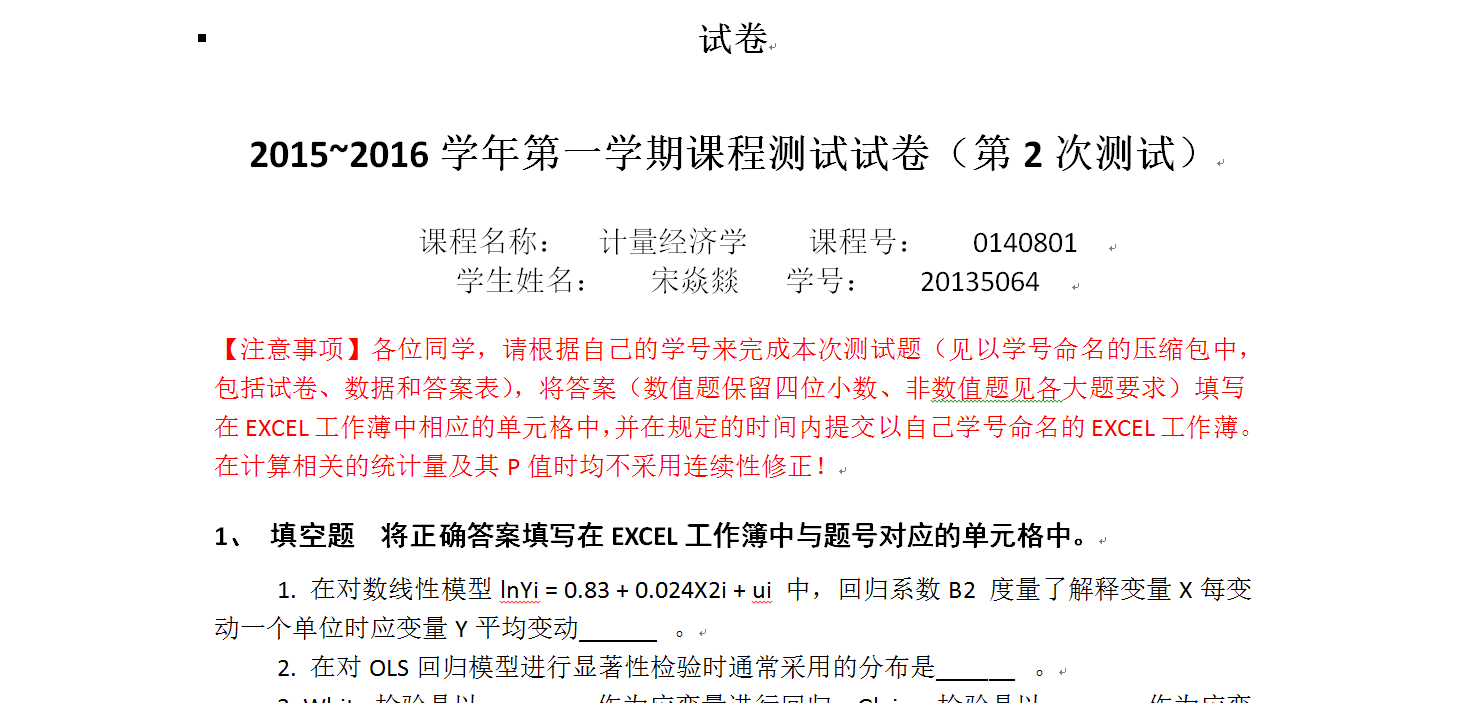
\includegraphics[height = 7cm]{images/shijuan.png}
            \caption{生成的试卷}
            \label{生成的试卷}
            \end{figure}

        \subsubsection{答案、答题卡和压缩文件}
            \begin{figure}
                \centering
                \begin{subfigure}[b]{0.4\textwidth}
                    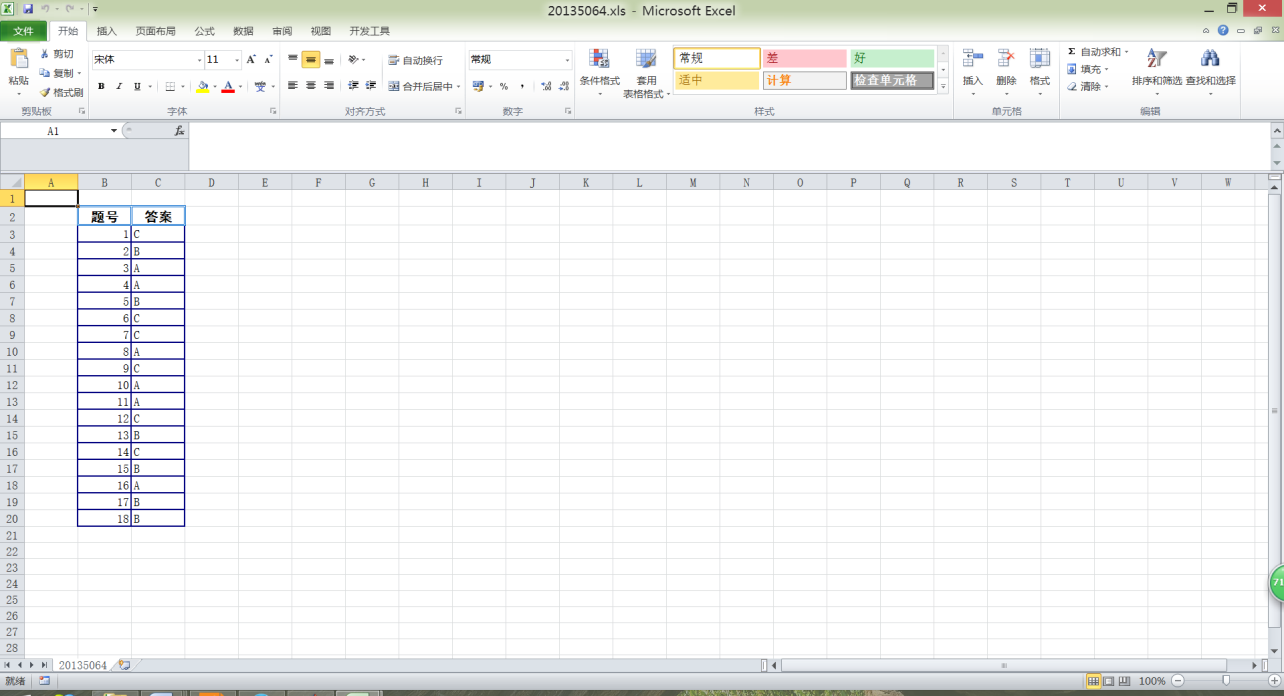
\includegraphics[width=\textwidth]{images/answer.jpg}
                    \caption{}
                    \label{fig:答案}
                \end{subfigure}
                \begin{subfigure}[b]{0.4\textwidth}
                    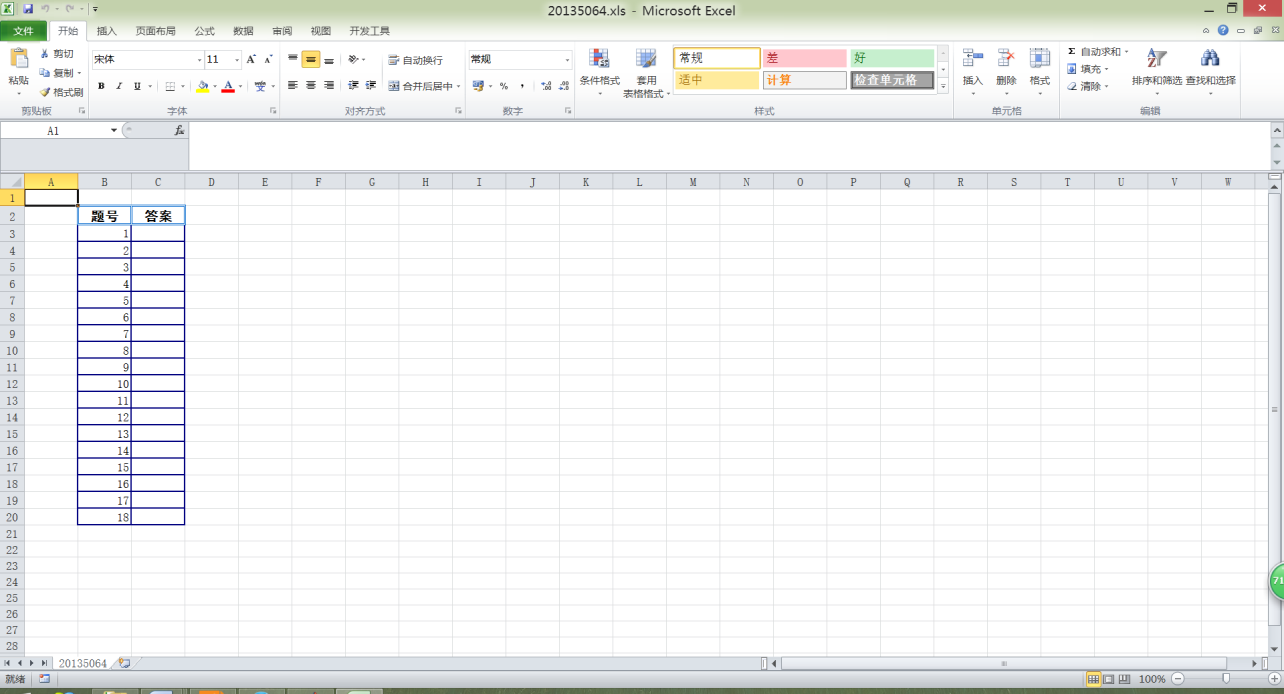
\includegraphics[width=\textwidth]{images/answer_card.jpg}
                    \caption{}
                    \label{fig:答题卡}
                \end{subfigure}
            % \quad
                \begin{subfigure}[b]{0.5\textwidth}
                    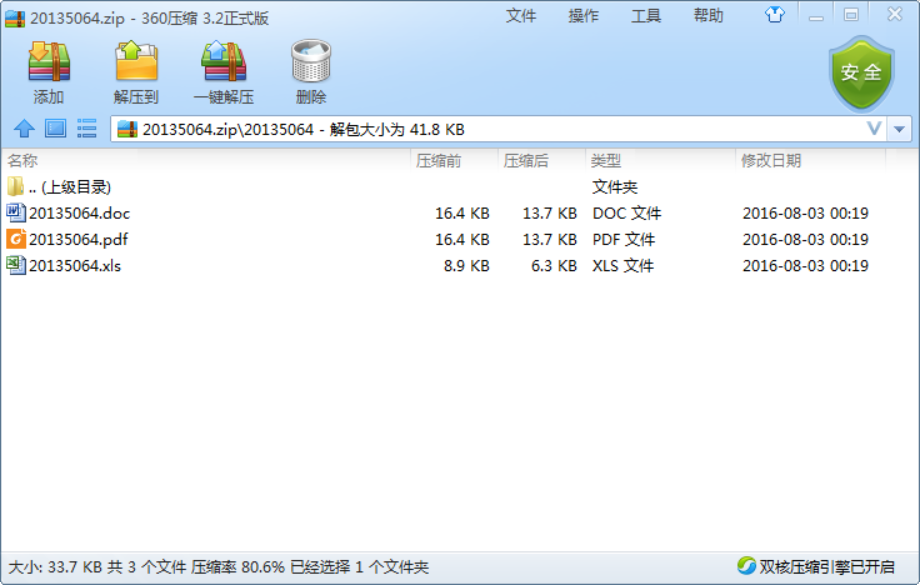
\includegraphics[width=\textwidth]{images/compressed_files.jpg}
                    \caption{}
                    \label{fig:压缩文件}
                \end{subfigure}
                 \caption{答案、答题卡和压缩文件}
            \end{figure}
            \par
            通过matlab将试卷or答案发送到邮箱
\section{matlab link R}
    \par
    这里我们使用R-link工具包来实现MATLAB链接R。首先,我们需要安装一些工具,安装过程如下:
    \par
    (1).安装R,这当然是必须的了\footnote{http://cran.r-project.org/}\footnote{https://www.rstudio.com/products/rstudio/download-server-2/}。
    \par
    (2).下载并安装Rcom server(这一步是至关重要的)\footnote{https://cran.r-project.org/contrib/extra/dcom/00ReadMe.html}\footnote{http://homepage.univie.ac.at/erich.neuwirth/php/rcomwiki/doku.php?id=wiki:how\_to\_install\#further\_remarks}\footnote{http://www.statconn.com/}\footnote{http://rcom.univie.ac.at/download.html\#RPackages\_rcom}。
    R (D)COM Server and RExcel 介绍如下:
    \par
    This package contains a DCOM server used to connect a client application (e.g. Microsoft Excel) with R.
    \par
    R (D)COM Server provides a COM-Interface to R as well as various COM objects and Active X controls for your applications. Additionally, an Add-In for Microsoft Excel is provided to easily use R in Excel and create statistical applications with Excel as the main GUI. The main features of this package are:
    \par
        COM server for local and remote use of R
        transfer of data into/from R, including NA, NaN,...
        Active X Controls for text and graphics output
        Installation/Uninstallation
        Repository for R instances for shared and exclusive access
        Many Samples
        Excel Add-In
    \par
    For more information see the documentation installed with the R (D)COM Server and visit the project's home page at http://sunsite.univie.ac.at/rcom.
    Author(s)
    \par
    Thomas Baier and Erich Neuwirth
    \begin{lstlisting}[language = R]
    # 用管理员身份运行R or Rstudio
    options(install.packages.check.source = "no")
    install.packages(c("rscproxy","rcom"),repos="http://rcom.univie.ac.at/download",lib=.Library,type="win.binary")
    library(rcom)
    comRegisterRegistry()
    \end{lstlisting}
    程辑包‘rscproxy’是用R版本3.2.2(这里一定要注意R版本的要求)\footnote{https://cran.r-project.org/src/base/R-3/} 来建造的;
    \par
    % Dcom Server需要在系统的Path中能够找到rproxy.dll和R.dll两个文件,R.dll一般直接安装R时机有即有,而rproxy.dll在 R2.7.0以后的版本中不再使用,变为rpcproxy.dll,而且需要手动安装rpcproxy包才会有,安装rpcproxy包后,需要将rpcproxy.dll所在目录手动添加到系统path中,比如我安装完后,rpcproxy.dll在C:\Program Files\R\R-2.9.0\library\rscproxy\libs中。
    \par
    (3).下载MATLAB R-link\footnote{http://cn.mathworks.com/matlabcentral/fileexchange/5051-matlab-r-link?s$\_$tid=srchtitle}
    并把里面的m文件复制到MATLAB的工作目录下;
    \par
    (4).加载rcom包,注意,在MATLAB中调用R时,一定要打开R加载rcom(r-GUI下,程序包-安装程序包,从里面找到rcom);
    \par
    (5).用MATLAB R-link里面的m文件试验一下
    \begin{lstlisting}[language = Matlab]
    %% Connecting MATLAB to R
    % The statistical programming language R has a COM interface. We can use
    % this to execute R commands from within MATLAB.
    %% Connect to an R Session
    openR
    %% Push data into R
    a = 1:10;
    putRdata('a',a)
    %% Run a simple R command
    b = evalR('a^2')
    %% Run a series of commands and grab the result
    evalR('b <- a^2');
    evalR('c <- b + 1');
    c = getRdata('c')
    %% Close the connection
    closeR
    \end{lstlisting}
    \par
    MATLAB R - link基于COM接口,允许我们在MATLAB中调用R函数,可调用的函数如表(\ref{R-link函数命令})所示
    \begin{table}[H]
    \caption{R-link函数命令}
    \label{R-link函数命令}
    \centering
    \begin{tabular}{c|l}
        \toprule
        命令 & 说明  \\
        \midrule
        openR&     连接到一R个服务器进程\\
        evalR&     运行R命令\\
        getRdata&  R变量复制到MATLAB\\
        putRdata&  MATLAB数据复制到一个R变量中\\
        closeR&    关闭R进程服务器\\
        Rdemo&     在MATLAB里利用R的一个例子\\
        \bottomrule
    \end{tabular}
    \end{table}
    MATALB R - link中使用了R的COM接口StatConnectorSrv.StatConnector,如下
    \begin{lstlisting}[language = Matlab]
    R_lInK_hANdle = actxserver('StatConnectorSrv.StatConnector');
    R_lInK_hANdle.Init('R');
    \end{lstlisting}
    我们将R的COM打开,如图(\ref{MATLAB-R接口})所示,由此我们可以据此来设计其它的link方法。
    \begin{figure}[H]
    \centering
    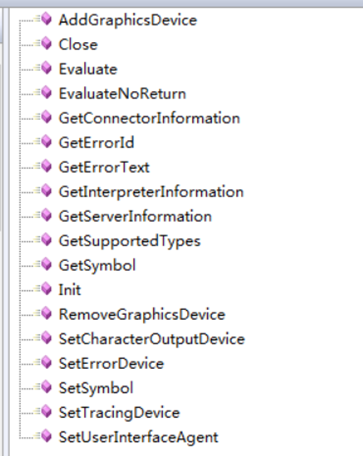
\includegraphics[height = 7cm]{images/MATLAB-Rjiekou.png}
    \caption{R COM接口}
    \label{MATLAB-R接口}
    \end{figure}

\section{matlab link python}
    \par
    MATLAB从R2014b开始就可以调用Python了\footnote{http://cn.mathworks.com/help/matlab/getting-started\_buik\_wp-3.html}。Python的某些库比MATLAB要好用,因此,MATLAB和Python的互相调用是必不可少的事情。下面,我们来介绍用MATLAB调用Python。
    \subsection{系统配置需求}
        \par
        在MATALB中调用Python时需要特定的Python版本, MATLAB(2014)支持的Python版本有2.7、3.3、3.4(这里不仅要注意Python的版本,还要注意Python是32位还是64位)。高版本的MATLAB应该已经支持所有Python版本了。 如果有版本限制,我们可以使用 pyversion 函数确定系统的版本。我们不能在一个MATLAB会话时切换Python的版本。 如果你想改变版本,重启MATLAB,然后运行pyversion version或pyversion executable(for Windows)。注意: 如果你下载一个Python解释器,但没有在Windows注册表中登记它,要使用pyversion executable来设置Python的版本。pyversion 查看和改变python解释器,其语法(Syntax)如下
        \begin{lstlisting}[language = Matlab]
          pyversion %查看Python的信息,返回结果如下:
          >>>  version: '2.7'
            executable: 'C:\Python27\python.exe'
               library: 'C:\windows\system32\python27.dll'
                  home: 'C:\Python27'
              isloaded: 0
          [version, executable(可执行的), isloaded] = pyversion% 返回Python的信息
          [version, executable, isloaded] = pyversion version % 设置Python的路径
          [version, executable, isloaded] = pyversion executable %设置Python的路径
        \end{lstlisting}

    \subsection{Python的基本使用}
        \subsubsection{Python的帮助函数}
            \par
            查看Python的帮助
            \begin{lstlisting}[language = Matlab]
            % 包的帮助
            py.help('textwrap')
            % 类的帮助
            py.help('textwrap.TextWrapper'
            % 类的方法的帮助
            py.help('textwrap.TextWrapper.wrap')
            % 函数的帮助
            py.help('textwrap.fill')
            \end{lstlisting}
        \subsubsection{调用用户定义的Python模块}
            \par
            复制下面这些命令并保存文件 mymod.py
            \begin{lstlisting}[language= Python]
            # mymod.py
            """Python module demonstrates passing MATLAB types to Python functions"""
            def search(words):
                """Return list of words containing 'son'"""
                newlist = [w for w in words if 'son' in w]
                return newlist
            def theend(words):
                """Append 'The End' to list of words"""
                words.append('The End')
                return words
            \end{lstlisting}
            \par
            添加当前文件夹于Python搜索路径
            \begin{lstlisting}[language = Matlab]
            f count(py.sys.path,'') == 0
                insert(py.sys.path,int32(0),'');
            end
            N = py.list({'Jones','Johnson','James'})
            names = py.mymod.search(N)
            \end{lstlisting}
            \par
            重新加载修改用户定义的Python模块,拷贝 myfunc 函数并保存文件 mymod.py 。
            \begin{lstlisting}[language = Python]
            def myfunc():
            """Display message."""
            return 'version 1'
            \end{lstlisting}
            \par
            重新加载修改用户定义的Python模块
            \begin{lstlisting}[language = Matlab]
            py.mymod.myfunc    %调用 myfunc
            clear classes   %卸载模块
            mod = py.importlib.import_module('mymod');   %导入修改模块
            py.reload(mod); %重新加载模块(在Python 2.7版本)
            py.imp.reload(mod); %重新加载模块(在Python 3.3版本)
            py.importlib.reload(mod); % 重新加载模块(在Python 3.4版本)
            py.mymod.myfunc  %在更新模块中调用函数(如果模块中的函数被修改)
            \end{lstlisting}
        \subsubsection{Python import and MATLAB import Commands}
            \par
            \begin{lstlisting}[language = Matlab]
            import x.y   % from x import y
            %例如,导入Python textwrap 模块 wrap的文本块。
            S = py.textwrap.wrap('This is a string');
            % 等价于
            import py.textwrap.wrap
            S = wrap('This is a string');
            clear import
            \end{lstlisting}
        \subsubsection{捕获的Python异常错误信息matlab.exception.PyException}
            \par
            捕获错误和异常的命令如下
            \par
            e = matlab.exception.PyException(msgID,errMsg,excObj)\\
            其中:msgID - Message identifier(character vector); errMsg - Error message(character vector); excObj - Exception object(pythonclass); e - Exception object(exception object)。示例如下面程序所示,更多的关于捕获异常的例子参见\footnote{http://cn.mathworks.com/help/matlab/matlab\_prog/capture-information-about-errors.html}。
            \begin{lstlisting}[language = Matlab]
            try
              py.list('x','y',1)
            catch e
              e.message
              if(isa(e,'matlab.exception.PyException'))
                e.ExceptionObject
              end
            end
            %ans = Python Error: TypeError: list() takes at most 1 argument (3 given)
            ans = Python tuple with no properties.
             (<type 'exceptions.TypeError'>, TypeError('list() takes at most 1 argument (3 given)',), None)
            \end{lstlisting}
        \subsubsection{未定义的变量或函数“py”}
            \par
            当你输入py发生失败:Undefined variable "py" or function "py.command"时,可以进行如下的故障排查:
            \par
            1、Python没有安装。从 https://www.python.org/downloads下载并安装Python 。如果你运行一个64位版本的MATLAB, 下载一个64位版本的Python,被命名为“窗口 x86 - 64 MSI安装程序”。
            \par
            2、你安装了一个32位版本的Python 64位版本 MATLAB。
            \par
            3、MATLAB无法找到Python。可以使用pyversion 函数来指定Python的路径。例如
            \begin{lstlisting}[language = Matlab]
            pyversion C:\Users\uname\WinPython-64bit-3.3.2.1\python-3.3.2.amd64\python.exe
            \end{lstlisting}如果你下载一个Python解释器,但没有在Windows注册表中登记它,使用命令:pyversion executable指定Python的位置。
            \par
            4、有一个错误的用户定义的Python模块。 py.importlib.import\_module('mymod')用来测试你的模块 mymod包含错误类型。如果Python模块检测到一个错误,MATLAB显示器显示 Python的错误消息。另外,Python命令执行的命令 Python错误消息提示。修正错误后,访问更新模块,重启MATLAB,并将其添加到搜索路径。
            \par
            5、Python模块不是Python搜索路径。如果命令是一个有效的Python命令,我们要确保Python模块在Python搜索路径。为了测试模块 mymod 在搜索路径上,使用py.importlib.import\_module('mymod')。如果Python没有找到模块,MATLAB显示器 Python的错误消息。在文件夹中添加 mymod modpath :
            \begin{lstlisting}[language = Matlab]
            P = py.sys.path;
            if count(P,'modpath') == 0
                insert(P,int32(0),'modpath');
            end
            \end{lstlisting}
            \par
            6、模块名称冲突。Python试图在错误的模块执行命令。如果 命令 在一个用户定义的模块,确保模块名称与Python标准模块并不冲突。
        \subsubsection{Unsupported MATLAB Types}
            \par
            下面是一些Python不支持的MATLAB数据结构:1.Multidimensional(多维的) arrays(数组) (numeric(数), char, or cell);2.Structure arrays;3.Complex, scalar integers or arrays;4.Sparse arrays;5.Logical vectors;6.categorical;7.table;8.containers.Map;9.datetime types;10.MATLAB objects;11.meta.class (py.class).
        \subsubsection{Call Methods on Python Variables}
            \begin{lstlisting}[language = Matlab]
            P = py.sys.path;
            % 显示Python list 的方法:
            methods(P)
            >>> Methods for class py.list:
                append   count    display  ge       insert   lt       plus     reverse
                cell     details  eq       gt       le       mtimes   pop      sort
                char     disp     extend   index    list     ne       remove
            py.help('list.append') % 阅读append的文档
            >>> list.append = append(...)
                   L.append(object) -- append object to end
            append(P, pwd) % 添加当前文件夹的路径
            py.len(P)
            >>> ans =
                Python int with properties:
                         real: [1x1 py.int]
                  denominator: [1x1 py.int]
                         imag: [1x1 py.int]
                    numerator: [1x1 py.int]
                  11
            % 11 是这条路经下的文件夹的数量。
            \end{lstlisting}
        \subsubsection{Call Python eval Function}
            \par
            \begin{lstlisting}[language = Matlab]
            py.help('eval')  %阅读的帮助
            >>> Help on built-in function eval in module __builtin__:
                eval(...)
                    eval(source[, globals[, locals]]) -> value

                    Evaluate the source in the context of globals and locals.
                    The source may be a string representing a Python expression
                    or a code object as returned by compile().
                    The globals must be a dictionary and locals can be any mapping,
                    defaulting to the current globals and locals.
                    If only globals is given, locals defaults to it.
            % 创建一个Python dict 变量。
            workspace = py.dict(pyargs('x',1,'y',6))
            >>> workspace =
                Python dict with no properties.
                  {'y': 6.0, 'x': 1.0}
            % 对表达式求值。
            res = py.eval('x+y',workspace)
            >>> res = 7
            % 添加两个数字没有分配变量。 通过一个空 dict 价值 为 全局变量 参数。
            res = py.eval('1+6',py.dict)
            >>> res = 7
            \end{lstlisting}


    \subsection{Python和Matlab的数据结构}
        \subsubsection{字符串}
            \par
            在Python method中输入MATLAB的向量(变量)
            \begin{lstlisting}[language = Matlab]
            folder = fullfile(matlabroot,'help','examples'); % Create a MATLAB variable(变量) .
            F = py.os.listdir(folder)% MATLAB automatically(自动的) converts(转换) folder to the Python str type.
            >>> F =
                  Python list with no properties.
                    ['graphics', 'graphics2', 'matlab']
            \end{lstlisting}
            在MATLAB中使用Python str类型(这个例子说明matlab和python的str不是同一class)
            \begin{lstlisting}[language = Matlab]
            p = py.os.path.pathsep
            c = pathsep
            c = ;
            isequal(class(p),class(c)) % Compare the MATLAB variable(变量的) type to the Python type.
            ans = 0 %A py.str type is not equivalent(等价的) to a MATLAB char type.
            f = ['myfile' char(p)] %Convert p to a MATLAB type and append(附加) the character to a file name.
            f = myfile;
            \end{lstlisting}
            Python字符串的索引
            \begin{lstlisting}[language = Matlab]
            str = 'myfile';% Create a MATLAB character vector and display the first character.
            str(1)
            ans = m
            pstr = py.str(str); %Convert(转变) the character vector to a Python str type and display the first character.
            pstr(1)
            ans = Python str with no properties.
            m
            \end{lstlisting}
            通过MATLAB反斜杠控制字符
            \begin{lstlisting}[language = Matlab]
            py.str(sprintf('The rain\nin Spain.'))% Python replaces \n with a new line.
            >>> ans =
                  Python str with no properties.
                    The rain
                    in Spain.
            py.str('The rain\nin Spain.')% Without the sprintf function, both MATLAB and Python interpret(说明) \ as a literal(文字的) backslash(反斜杠).
            >>> ans =
                  Python str with no properties.
                    The rain\nin Spain.
            split(py.str('The rain\nin Spain.'))% Pass this string to a Python string method, split.
            >>> ans =
                  Python list with no properties.
                    ['The', 'rain\\nin', 'Spain.']
            \end{lstlisting}

        \subsubsection{列表}
            \par
            创建Python列表变量
            \begin{lstlisting}[language = Matlab]
            students = py.list({'Robert','Mary','Joseph'}) % 创建python列表变量
            >>> students =
                  Python list with no properties.
                    ['Robert', 'Mary', 'Joseph']
            n = py.len(students)# Display number of students in the list.
            >>> n = 3
            \end{lstlisting}
            在MATLAB中使用Python列表类型
            \begin{lstlisting}[language  = Matlab]
            P = py.sys.path;% Create a Python list
            class(P)
            >>> ans  =  py.list
            cP = cell(P); %Convert list P to a MATLAB type. The first step is to convert(转变) the list to a cell array(数组) of folder names, cP.
            class(cP)
            >>> ans =cell
            class(cP{1}) % Each folder name is a Python string.
            >>> ans =py.str
            cellP = cellfun(@char,cell(P),'UniformOutput',false); %create cellP using the cellfun function to combine the conversion(转换) functions.
            % Display the folder names.
            for n=1:py.len(P)
                disp(cellP{n})
            end
            \end{lstlisting}
            将Python数值类型列表转化为MATLAB double数组。
            Suppose that you have a Python function that returns the following list of integers, P.
            \begin{lstlisting}[language = Matlab]
            >>> P =
              Python list with no properties.
                [1, 2, 3, 4]
            % Display the numeric(数) type of the values.
            class(P{1})
            ans = int64
            cP = cell(P);% Convert P to a MATLAB cell array(数组).
            A = cellfun(@double,cP) % Convert(转变) the cell array to a MATLAB array of double.
            >>> A = 1     2     3     4
            \end{lstlisting}
            Python列表的索引
            \begin{lstlisting}[language = Matlab]
            C = {1,2,3,4};
            n = C(end)
            n = [4] %MATLAB returns a cell array.
            n = C{end}% Display the contents of the last element.
            >>> n = 4
            li = py.list(C) %Convert(转变) the cell array to a Python list.
            >>> li =
                  Python list with no properties.
                    [1.0, 2.0, 3.0, 4.0]
            n = li(end)  %Display the last element. returns a list.
            >>> n =
                  Python list with no properties.
                    [4.0]
            n = li{end}% Display the contents of the last element.
            >>> n = 4
            \end{lstlisting}
            在for循环中display Python列表值
            \begin{lstlisting}[language = Matlab]
            li = py.list({1,2,3,4});
            for n = li
                disp(n{1})
            end
            \end{lstlisting}
            This example shows how to pass a MATLAB cell array to a Python function. 将下面的程序保存为mymod.py
            \begin{lstlisting}[language = Python]
            # mymod.py
            """Python module demonstrates passing MATLAB types to Python functions"""
            def search(words):
                """Return list of words containing 'son'"""
                newlist = [w for w in words if 'son' in w]
                return newlist
            def theend(words):
                """Append 'The End' to list of words"""
                words.append('The End')
                return words
            \end{lstlisting}
            \begin{lstlisting}[language = Matlab]
            P = py.sys.path;
            append(P,prefdir);% Add the folder containing mymod.py to the Python search path using the append method of the list type.
            load patients.mat
            L = py.list(LastName'); %Convert(转变) the cell array to a 1-by-N py.list array.
            class(L)
            >>> ans = py.list
            py.mymod.theend(L); %Call mymod.theend on the list.
            L{end}
            >>> ans =
                  Python str with no properties.
                   The End
            \end{lstlisting}
            读取嵌套列表类型的元素
            \begin{lstlisting}[language = Matlab]
            matrix = py.list({{1, 2, 3, 4},{'hello','world'},{9, 10}});
            disp(char(matrix{2}{2}))% Display element 'world', at index (2,2).
            %% 显示元素的范围
            li = py.list({'a','bc',1,2,'def'});
            li(1:2:end)
            \end{lstlisting}

        \subsubsection{元组tuple}
            \par
            \begin{lstlisting}[language = Matlab]
            % 1.创建Python tuple变量
            student = py.tuple({'Robert',19,'Biology'})
            % 2.在MATLAB中使用Python tuple类型
            pn = py.os.path.split('C:\Program Files\MATLAB\R2014a\help\examples')
            head = char(pn{1})
            tail = char(pn{end})
            head =C:\Program Files\MATLAB\R2014a\help
            tail = examples
            % 3.Python Tuple索引
            t = py.tuple({'a','bc',1,2,'def'});
            t(1:2)
            % 4.创建单个Python tuple变量 (只包含一个元素的tuple)
            subject = py.tuple({'Biology'})
            \end{lstlisting}

        \subsubsection{字典dict}
            \par
            \begin{lstlisting}[language = Matlab]
            % 1.创建Python dict类型变量
            studentID = py.dict(pyargs('Robert',357,'Mary',229,'Jack',391))
            % 2.在MATLAB中使用Python dict类型
            keys(studentID) % Use the Python keys function to display the menu items.
            values(studentID) % Use the Python values function to display the prices.
            p = cell(values(studentID))% Use the cell function to convert the Python list to a MATLAB variable.
            prices = cellfun(@double,p)%Convert the prices to a MATLAB array.
            total = sum(prices)%Calculate the total.
            % 3.索引Python dict类型
            customers = py.dict %Create a dictionary variable(变量).
            customers{'Smith'} = int32(2112);
            customers{'Anderson'} = int32(3010);
            customers{'Audrey'} = int32(4444);
            customers{'Megan'} = int32(5000);
            acct = customers{'Anderson'}
            acct = 3010
            class(acct)
            >>> ans = double
            % 4.change a value in a dict variable using the Python update method.
            menu = py.dict(pyargs('soup',3.57,'bread',2.29,'bacon',3.91,'salad',5.00));
            update(menu,py.dict(pyargs('bread',2.50))) %Update the price for bread using the Python dict type update method.
            % 5.Python dict类型转换为MATLAB结构
            patient % Suppose a Python function returns a variable, patient, with the following values.
            >>> patient =
                    Python dict with no properties.
                      {'test1': array('d', [79.0, 75.0, 73.0]),
                       'test3': array('d', [220.0, 210.0, 205.0]),
                       'test2': array('d', [180.0, 178.0, 177.5]),
                       'name': 'John Doe'}
            P = struct(patient) %Convert patient to a MATLAB structure.
            >>> P =
                    test1: [1x1 py.array.array]
                    test3: [1x1 py.array.array]
                    test2: [1x1 py.array.array]
                     name: [1x8 py.str]
            \end{lstlisting}
        \subsubsection{numbers}
            \par
            \begin{lstlisting}[language = Matlab]
            % 1.在MATLAB使用Python数值类型
            pynum = py.math.radians(90)
            class(pynum)% MATLAB automatically(自动的) converts(转化) Python float type to double.
            % 2.调用Python方法与数值参数
            load patients.mat
            class(Height)
            >>> ans =double
            size(Height)
            >>> ans = 100     1
            py.math.fsum(Height')% Transform Height to a 1-by-N matrix before calling fsum.
            >>> ans =6707
            % 3.在MATLAB中使用Python数组类型
            P = %Suppose(假设) that you have a Python function that returns the following array, P
                Python array with properties:
                itemsize: 8
                typecode: [1x1 py.str]
                array('d', [1.0, 2.0, 3.0, 4.0, 5.0])
            A = double(P); %Convert P to a MATLAB array of type double.
            sum(A) % Sum the elements of A.
            >>> ans =5
            \end{lstlisting}
        \subsubsection{关键字}
            \par
            \begin{lstlisting}[language = Matlab]
            %% The Python built-in print function has keyword arguments, sep, end, and file.
            print(*objects, sep=' ', end='\n', file=sys.stdout)
            % The following examples use the default value for file.
            % Create some text variables(变量).
            x1 = py.str('c:');
            x2 = py.os.curdir;
            x3 = py.os.getenv('foo');
            py.print(x1,x2,x3)
            >>> c: . None
            % To display the values on separate lines, use newline, \n, as a separator(分离器).
            py.print(x1,x2,x3,pyargs('sep',sprintf('\n')))
            >>> c:
                .
                None
            % Use the following statement(声明) to change sep to an empty string and change the end value to display THE END.
            py.print(x1,x2,x3,pyargs('end', sprintf(' THE END\n'),'sep',py.str))
            >>> c:.None THE END
            \end{lstlisting}
        \subsubsection{函数}
            \par
            This example shows how to display the length of each word in a list.
            \begin{lstlisting}[language = Matlab]
            days = py.list({'Monday','Tuesday','Wednesday','Thursday','Friday'}); %Create a list of days of the work week.
            % Apply the Python len function to the py.map function to display the length of each word. Use the MATLAB function handle notation(符号), @, to indicate py.len is a function.
            py.map(@py.len,days)
            >>> ans =
                Python list with no properties.
                  [6, 7, 9, 8, 6]
            % Python version 2.7 returns a list.
            % Python versions 3.x return a map object. To display the contents, type:
            py.list(py.map(@py.len,days))
            >>> ans =
                  Python list with no properties.
                    [6, 7, 9, 8, 6]
            \end{lstlisting}
    \subsection{MATLAB和Python之间的转换}
        \subsubsection{MATLAB与Python在创建列表、元组、字典之间的差异}
            The following table(\ref{the commands for creating list, tuple, and dict types}) shows the commands for creating list, tuple, and dict types. The commands on the left are run from the Python interpreter(解释者). The commands on the right are MATLAB commands.
            \begin{table}[htbp]
              \centering
              \caption{the commands for creating list, tuple, and dict types}
              \label{the commands for creating list, tuple, and dict types}
              \begin{tabular}{l|l}
                \toprule[1pt]
                Python & Matlab\\
                \midrule
                \rowcolor[gray]{0.9}  Python list - [] & MATLAB py.list\\
                $['Robert', 'Mary', 'Joseph'] $& $py.list(\{'Robert','Mary','Joseph'\})$\\
                $[[1,2],[3,4]]$& $py.list(\{py.list([1,2]),py.list([3,4])\})$\\
                \rowcolor[gray]{0.9}  Python tuple - ()& MATLAB py.tuple\\
                $('Robert', 19, 'Biology')$ &$py.tuple (\{'Robert',19,'Biology'\})$\\
                \rowcolor[gray]{0.9}  Python dict - $\{\}$ & MATLAB py.dict\\
                $\{'Robert': 357, 'Joe': 391, 'Mary': 229\}$ & $py.dict(pyargs('Robert',357,'Mary',229,'Joe',391))$\\
                \bottomrule[1pt]
              \end{tabular}
            \end{table}
        \subsubsection{MATLAB Type to Python Type Mapping}
            When you pass MATLAB data as arguments to Python, MATLAB converts the data into types that best represent the data to the Python language 表(\ref{MATLAB Type to Python Type Mapping}).
            \begin{table}[htbp]
              \centering
              \caption{MATLAB Type to Python Type Mapping}
              \label{MATLAB Type to Python Type Mapping}
              \begin{tabular}{l|l}
              \toprule
              MATLAB Input Argument Type - Scalar Values Only& Resulting Python Type \\
              \midrule
              double single & float\\
              Complex single Complex double & complex\\
              int8 uint8 int16 uint16 int32 & int\\
              uint32 int64 uint64 & int long(onlyversion2.7)\\
              NaN& float(nan)\\
              Inf &float(inf)\\
              logical &bool\\
              Structure& dict\\
              Python object - py.type& type\\
              function handle $@$py.module.function, to Python functions only & module.function\\
              \bottomrule
              \end{tabular}
            \end{table}
        \subsubsection{处理从Python回来的数据}
            Automatic(自动的) Python Type to MATLAB Type Mapping The following table shows how MATLAB converts data returned from Python into MATLAB types 表(\ref{处理从Python回来的数据}).
            \begin{table}[H]
              \centering
              \caption{处理从Python回来的数据}
              \label{处理从Python回来的数据}
              \begin{tabular}{l|l}
              \toprule
              Python Return Type, as Displayed in Python& Resulting MATLAB Type - Scalar \\
              \midrule
              bool & logical\\
              int (version 2.7 only) & int64\\
              float & double\\
              complex & Complex double\\
              All other Python types - type& Python object - py.type\\
              \bottomrule
              \end{tabular}
            \end{table}

            MATLAB provides the following functions to convert Python data types to MATLAB types manually(手动地)表(\ref{处理从Python回来的数据2}).
            \begin{table}[H]
              \centering
              \caption{处理从Python回来的数据2}
              \label{处理从Python回来的数据2}
              \newcolumntype{Y}{>{\centering\arraybackslash}X}% 定义自适应列的居中格式 Y, 用 X 为左对齐(自适应列)
              \begin{tabularx}{\textwidth}{l|l}% 需要引入 tabularx 宏包;表格总宽度一定要设置
              \toprule
              Python Return Type or Protocol, as Displayed in MATLAB& MATLAB ConversionFunction \\
              \midrule
              py.str (version 2.7) & char uint8\\
              py.str (version 3.x) & char\\
              py.unicode & char\\
              Object with \_str\_ method & char\\
              py.bytes & uint8\\
              py.int & double or int64\\
              py.long& double or int64\\
              py.array.array& numeric double single int8\\
              py.array.array& uint8 int16 uint16 int32\\
              py.array.array& uint32 int64 uint64\\
              Sequence protocol; for example, py.list and py.tuple & cell\\
              Mapping protocol; for example, py.dict & struct\\
              \bottomrule
              \end{tabularx}
            \end{table}

\section{matlab link SQL}

\section{matlab link C java }

% \bibliography{part-matlab-chap-drawing}%bib文件名称
% \end{document}
